% -*- latex -*-

In this chapter you will learn the use of the main tool for 
distributed memory programming: the \acf{MPI} library.
The \ac{MPI} library has about 250 routines, many of which you may
never need. Since this is a textbook, not a reference manual, we will
focus on the important concepts and give the important routines for
each concept. What you learn here should be enough for most common
purposes. You are advised to keep a reference document handy, in
case there is a specialized routine, or to look up subtleties about
the routines you use.

\Level 0 {Distributed memory and message passing}

In its simplest form, a distributed memory machine is a bunch of 
single computers hooked up with network cables. In fact, this has a name:
a \indexterm{Beowulf cluster}. As you recognize from that setup, 
each processor will run an independent program, and has its own memory
without direct access to other processors' memory. MPI is the magic
that makes multiple instantiations of the same executable run
so that they know about each other and can exchange data through the 
network.

One of the reasons that MPI is so successful as a tool for high
performance on clusters is that it is very explicit: the programmer
controls many details of the data motion between the processors.
Consequently, a capable programmer can write very efficient code with MPI.
Unfortunately, that programmer will have to spell things out
in considerable detail. For this reason, people sometimes call MPI
`the assembly language of parallel programming'. If that sounds scary,
be assured that things are not that bad. You can get started 
fairly quickly with MPI, using just the basics,
and coming to the more sophisticated tools 
only when necessary.

Another reason that MPI was a big hit with programmers is that
it does not ask you to learn a new language: it is a library that 
can be interface to C/C++ or Fortran; there are even bindings to Python.
A~related point is that it is easy to install: there are free implementations
that you can download and install on any computer that has a Unix-like
operating system, even if that is not a parallel machine.

\Level 1 {History}

Mid 1990s, many parties involved, big concensus. Many competing packages
before, few after.

\Level 1 {Basic model}

Here we sketch the two most common scenarios for using MPI. In the
first, the user is working on an interactive machine, which has
network access to a number of hosts, typically a network of workstations;
see figure~\ref{fig:mpi-interactive}.
\begin{figure}[ht]
  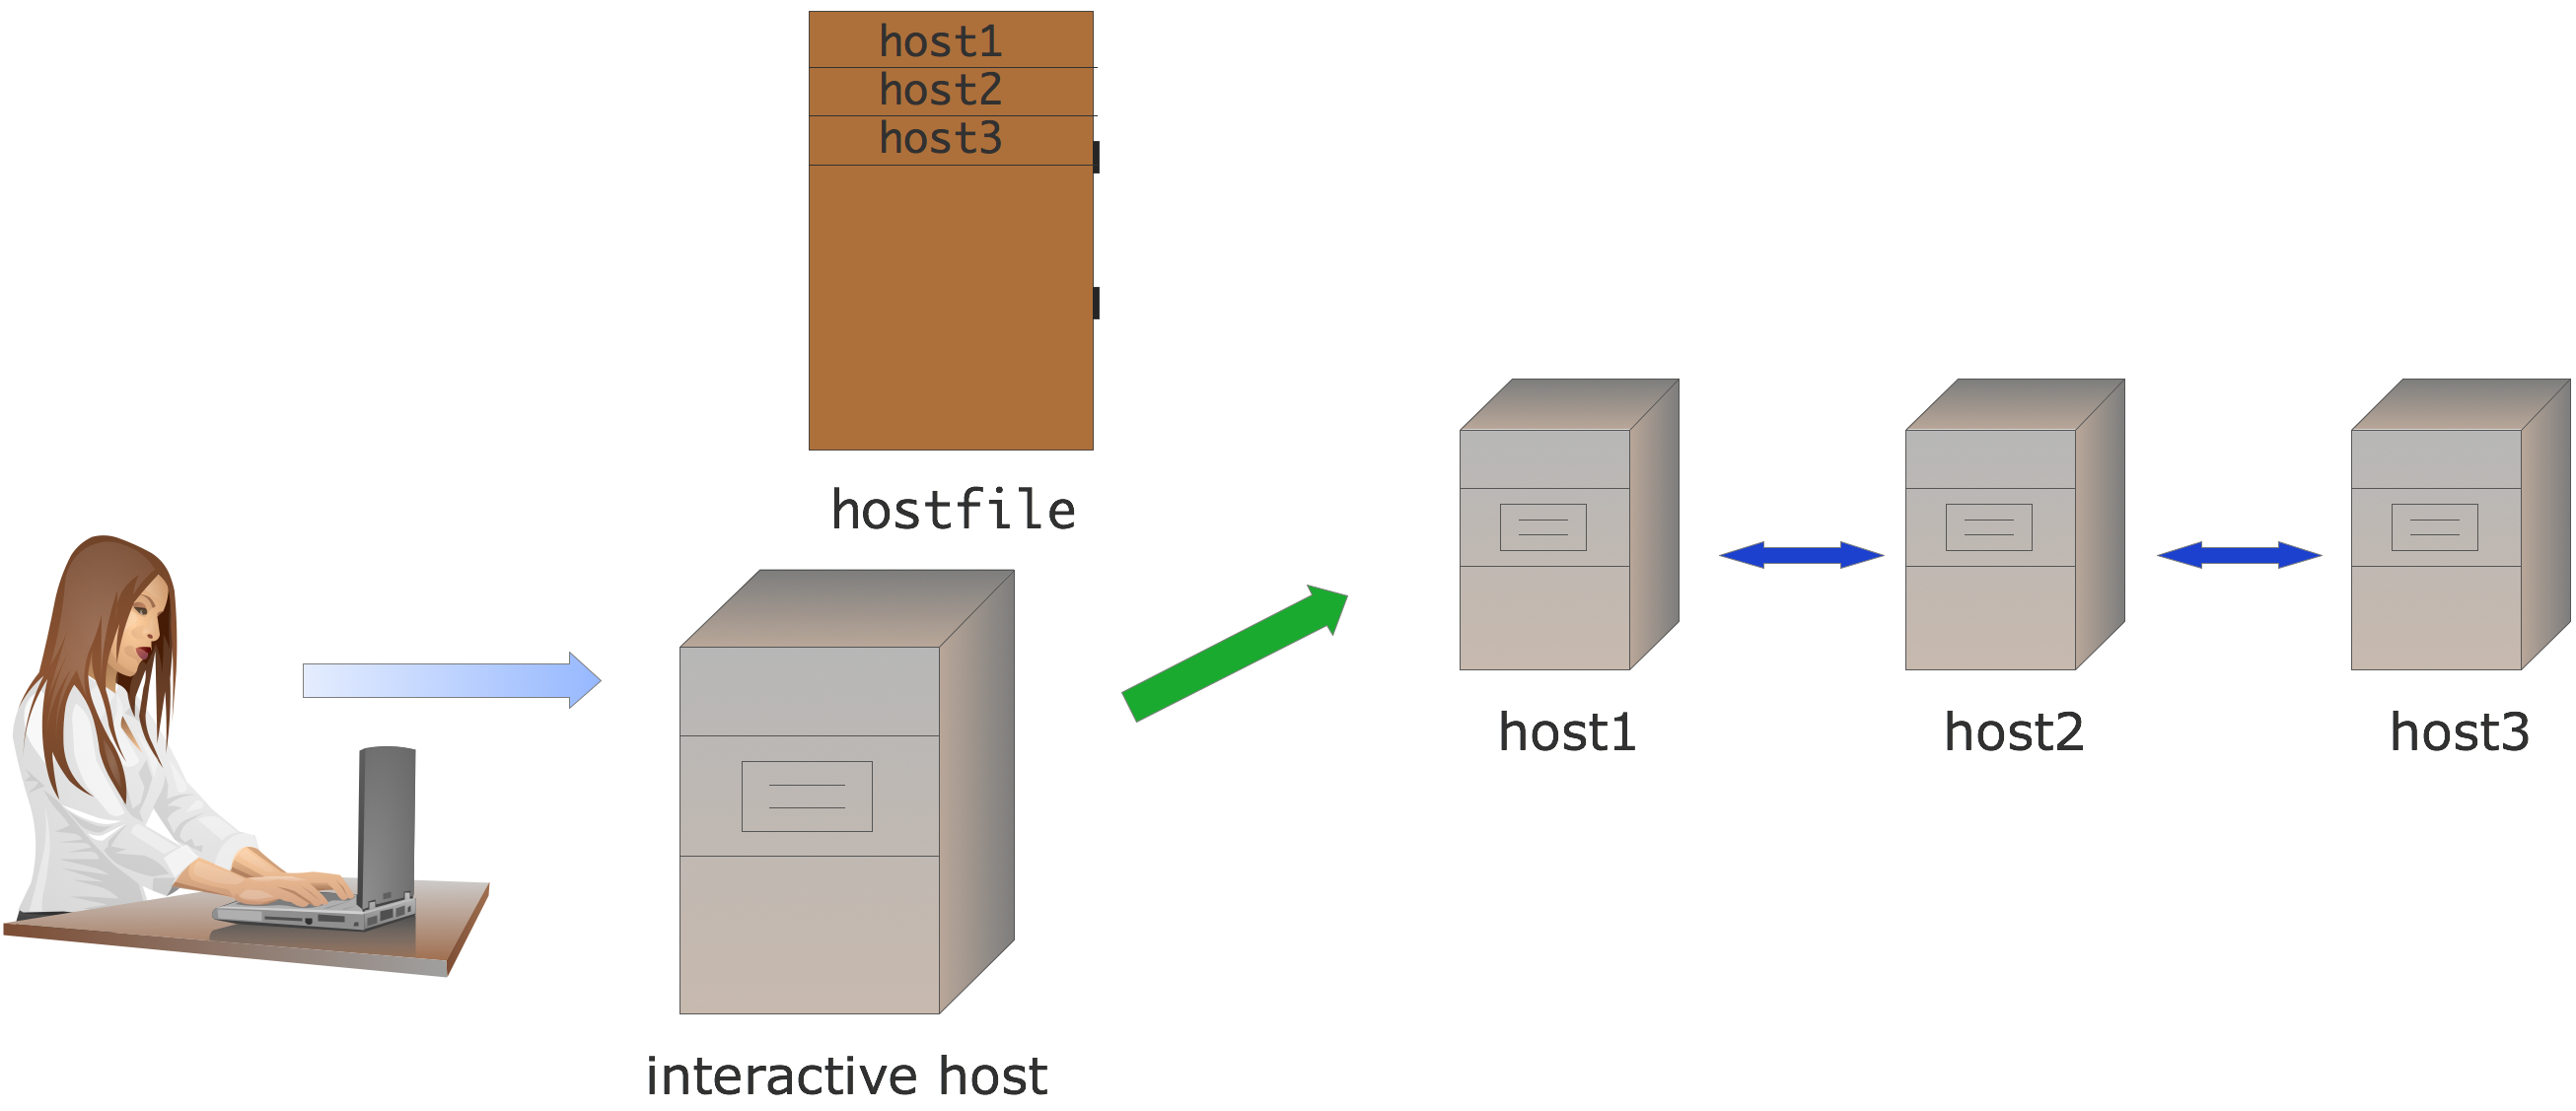
\includegraphics[scale=.12]{graphics-public/mpi-interactive}
  \caption{Interactive MPI setup}
  \label{fig:mpi-interactive}
\end{figure}
The user types the command \n{mpirun}\index{mpirun} and supplies
\begin{itemize}
\item The number of hosts involved,
\item their names, possibly in a hostfile,
\item and other parameters, such as whether to include the interactive
  host; followed by
\item the name of the program and its parameters.
\end{itemize}
The \n{mpirun} program then makes an \n{ssh}\index{ssh} connection
to each of the hosts, giving them sufficient information that they 
can find each other. All the output of the processors is piped through the 
\n{mpirun} program, and appears on the interactive console.

In the second scenario (figure~\ref{fig:mpi-batch}) the user prepares
a \indextermbus{batch}{job} script with commands, and these will be
run when the \indextermbus{batch}{scheduler} gives a number of hosts
to the job.
\begin{figure}[ht]
  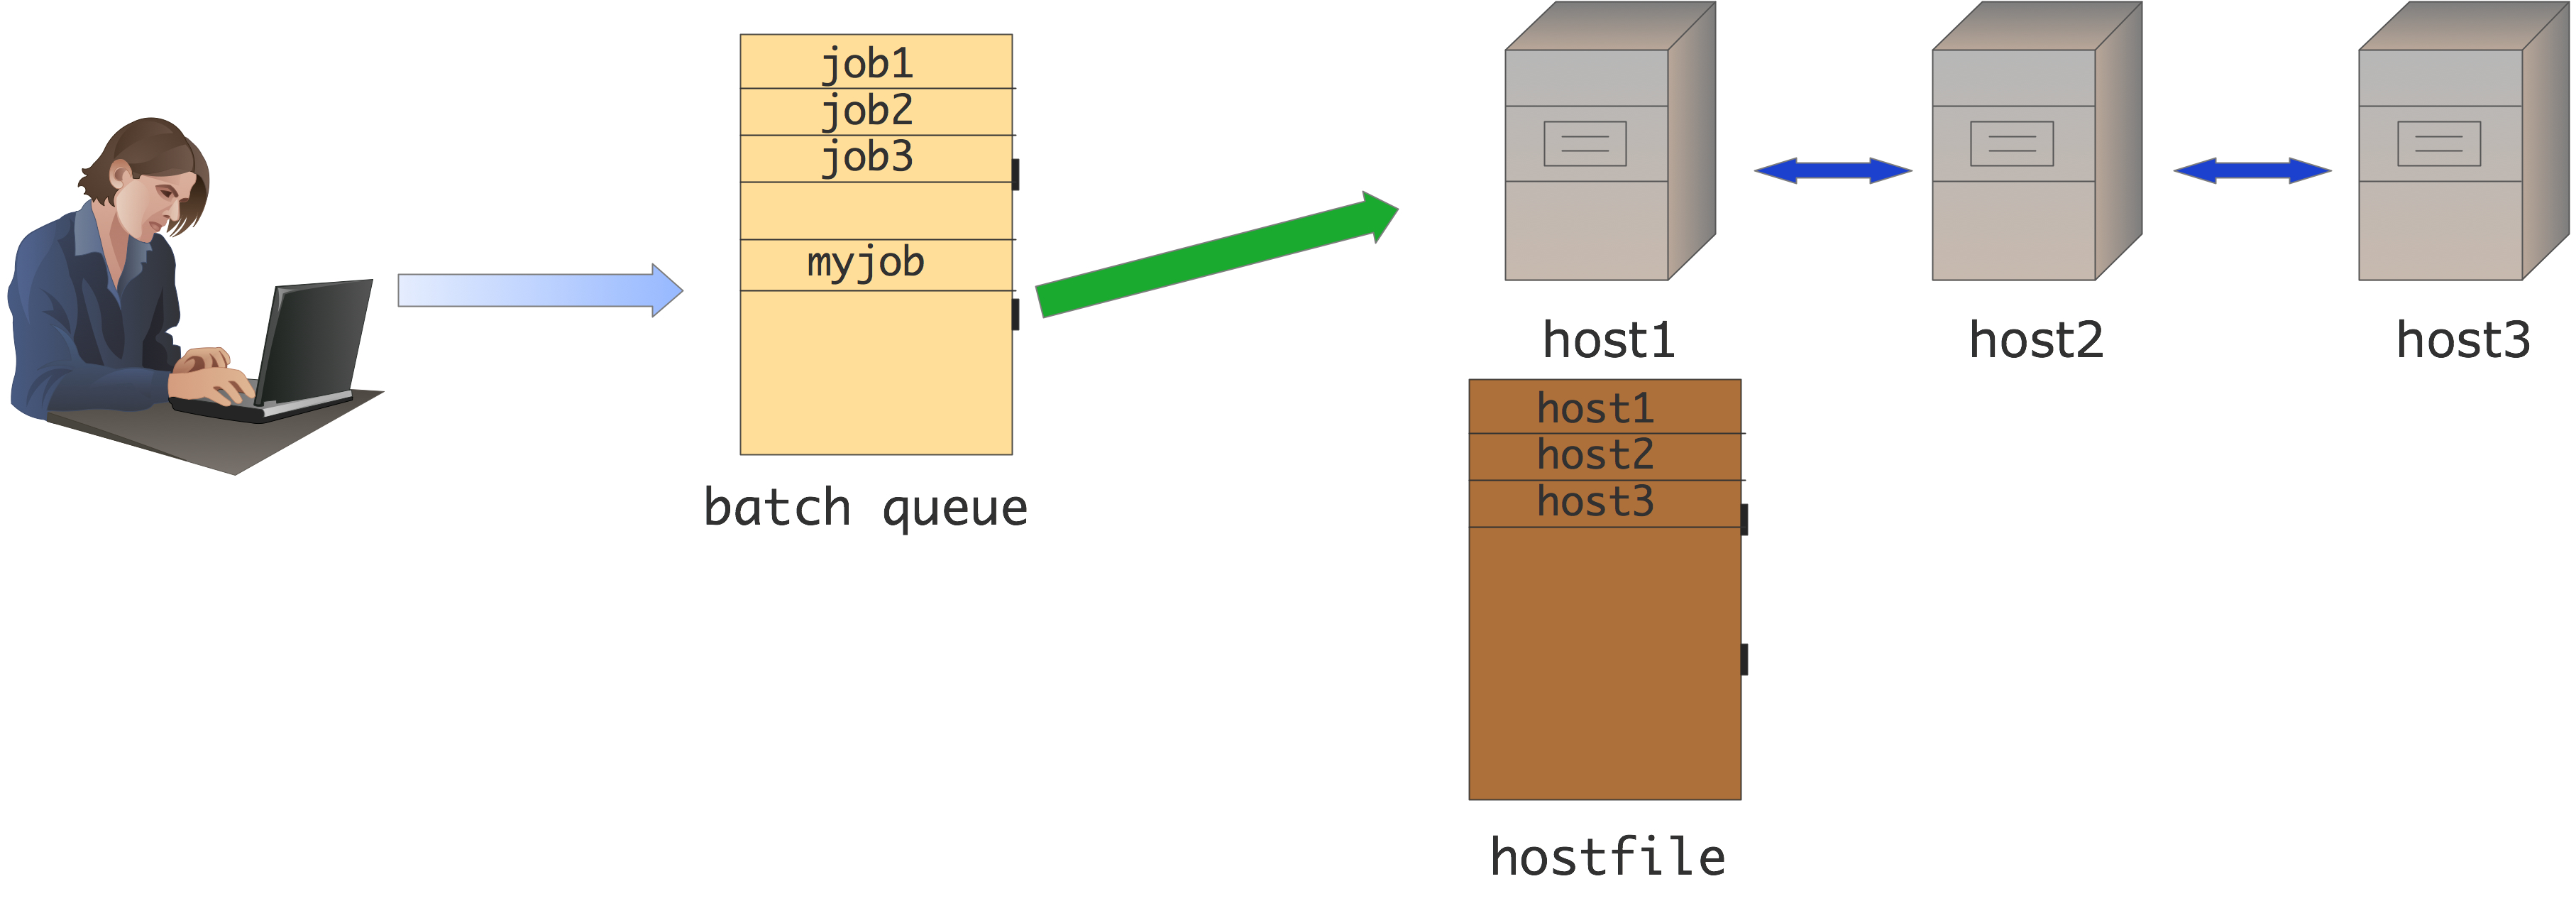
\includegraphics[scale=.1]{graphics-public/mpi-batch}
  \caption{Batch MPI setup}
  \label{fig:mpi-batch}
\end{figure}
Now the batch script contains the \n{mpirun} command%
\begin{istc}
, or some variant such as \n{ibrun}\index{ibrun}%
\end{istc}
, and the hostfile is dynamically generated when the job starts.
Since the job now runs at a time when the user may not be logged in, 
any screen output goes into an output file.

You see that in both scenarios the parallel program is started
by the \n{mpirun} command, which only supports
an \ac{SPMD} mode of execution: all hosts execute the same program.

To first order, the network is symmetric. However, the truth is more 
complicated (`topology-aware communication').

\Level 1 {Making and running an MPI program}

MPI is a library, called from programs in ordinary programming languages
such as C/C++ or Fortran. To compile such a program you use your regular
compiler:
\begin{verbatim}
gcc -c my_mpi_prog.c -I/path/to/mpi.h
gcc -o my_mpi_prog my_mpi_prog.o -L/path/to/mpi -lmpich
\end{verbatim}
However, MPI libraries may have different names between different
architectures, making it hard to have a portable makefile. Therefore,
MPI typically has shell scripts around your compiler call:
\begin{verbatim}
mpicc -c my_mpi_prog.c
mpicc -o my_mpi_prog my_mpi_prog.o
\end{verbatim}

MPI programs can be run on many different architectures. Obviously it
is your ambition (or at least your dream) to run your code on a
cluster with a hundred thousand processors and a fast network. But
maybe you only have a small cluster with
plain \indexterm{ethernet}. Or maybe you're sitting in a plane, with
just your laptop. An MPI program can be run in all these
circumstances~--~within the limits of your available memory of course.

The way this works is that you do not start your executable directly,
but you use a program, typically called \n{mpirun}\index{mpirun} or
something similar, which makes a connection to all available
processors and starts a run of your executable there. So if you have a
thousand nodes in your cluster, \n{mpirun} can start your program once
on each, and if you only have your laptop it can start a few instances
there. In the latter case you will of course not get great
performance, but at least you can test your code for correctness.

\Level 0 {Basic concepts}

\Level 1 {Initialization / finalization}
\commandref{sec:mpi-init}

Every program that uses MPI needs to initialize and finalize exactly
once. In~C, the calls are
\begin{verbatim}
ierr = MPI_Init(&argc,&argv);
// your code
ierr = MPI_Finalize();
\end{verbatim}
where \n{argc} and \n{argv} are the arguments of the main program.
%
The corresponding Fortran calls are
\begin{verbatim}
call MPI_Init(ierr)
// your code
call MPI_Finalize()
\end{verbatim}
(There is a call \indexmpishow{MPI_Abort} if you want to abort execution
completely.)

We make a few observations.
\begin{itemize}
\item MPI routines return an error code. In~C, this is a function
  result; in Fortran it is the final parameter in the calling
  sequence.
\item For most routines, this parameter is the only difference between
  the C and Fortran calling sequence, but some routines differ in some
  respect related to the languages. In this case, C~has a mechanism
  for dealing with commandline arguments that Fortran lacks.
\item This error parameter is zero if the routine completes
  succesfully, and nonzero otherwise. You can write code to deal with
  the case of failure, but by default your program will simply abort
  on any MPI error. See section~\ref{mpi:error} for more details.
\end{itemize}

The commandline arguments \n{argc} and \n{argv} are only guaranteed to
be passed to process zero, so the best way to pass commandline information
is by a broadcast (section~\ref{sec:bcast}).

\Level 1 {Communicators}
\label{sec:comm-intro}

Before we can discusss any further MPI routines we need to take a first look at an 
important concept: that of the \indexterm{communicator}. A~communicator
stands for a group of processes. Thus, almost all MPI routines have
a communicator argument: you can never ask how many processes there are, or 
send data to process~5, you have to ask how many processes in a given communicator,
or send data to process~5 in a communicator.

There are several reasons for having communicators. One is that sometimes you 
may want to divide your processes in two groups, each of which engages in a 
different activity. Another reason is for ease of writing software libraries.
If a software library that uses MPI starts by creating its own communicator,
even if it contains the same processes as the communicator in the calling program,
it can safely use that and never run the risk of confusion between messages 
in the library code and messages in the user code. We will discuss this in more detail
later on.

For most of your MPI programming, the only communicator you will use
is \indexmpishow{MPI_COMM_WORLD} which contains all your
processes. Later you will learn of the mechanisms for creating other
communicators from it.

\Level 1 {Distinguishing between processes}
\commandref{sec:rank-size}

In the SPMD model you run the same executable on each of a set of
processors; see section~\HPSCref{sec:spmd}. So how can you do anything
useful if all processors run the same code? Here is where your first
two MPI routines come in,
which query the 
\n{MPI_COMM_WORLD} communicator and each process' place in it.

With \indexmpishow{MPI_Comm_size} a processor can query how many
processes there are in total, and with \indexmpishow{MPI_Comm_rank} it
can find out what its number is. This rank is a number from zero to
the comm size minus~one. (Zero-based indexing is used even if you
program in Fortran.)

Using these calls, the simplest MPI programs does this:
\verbatimsnippet{hello}

\Level 0 {Point-to-point communication}

MPI has two types of message passing routines: point-to-point and
collectives. In this section we will discuss point-to-point
communication, which involves the interaction of a unique sender and a
unique receiver. Collectives, which involve all processes in some
joint fashion, will be discussed in the next section.

There is a lot to be said about simple sending and receiving of
data. We will go into three broad categories of operations: blocking
and non-blocking two-sided communication, and the somewhat
more tricky one-sided communication.

Two-sided communication is a little like email: one party send data, 
which needs to be specified, to another party. The other party can then
be expecting a message from a specified sender or it can be open
to receiving from any source, but in either case the receiver
indicates that something is to be expected. 
One-sided communication is very different in nature. Compare it to leaving your
front-door open and people can bring things to your house, or take them,
without you noticing.

\Level 1 {Blocking communication}
\index{communication!two-sided|(}
\index{communication!blocking|(}
\commandref{sec:blocking}

In two-sided communication, one process issues a send call and the
other a receive call. Life would be easy if the send call put the data
somewhere in the network for the receiving process to find whenever it
gets around to its receive call. This ideal scenario is pictured
figure~\ref{fig:send-ideal}.
\begin{figure}[ht]
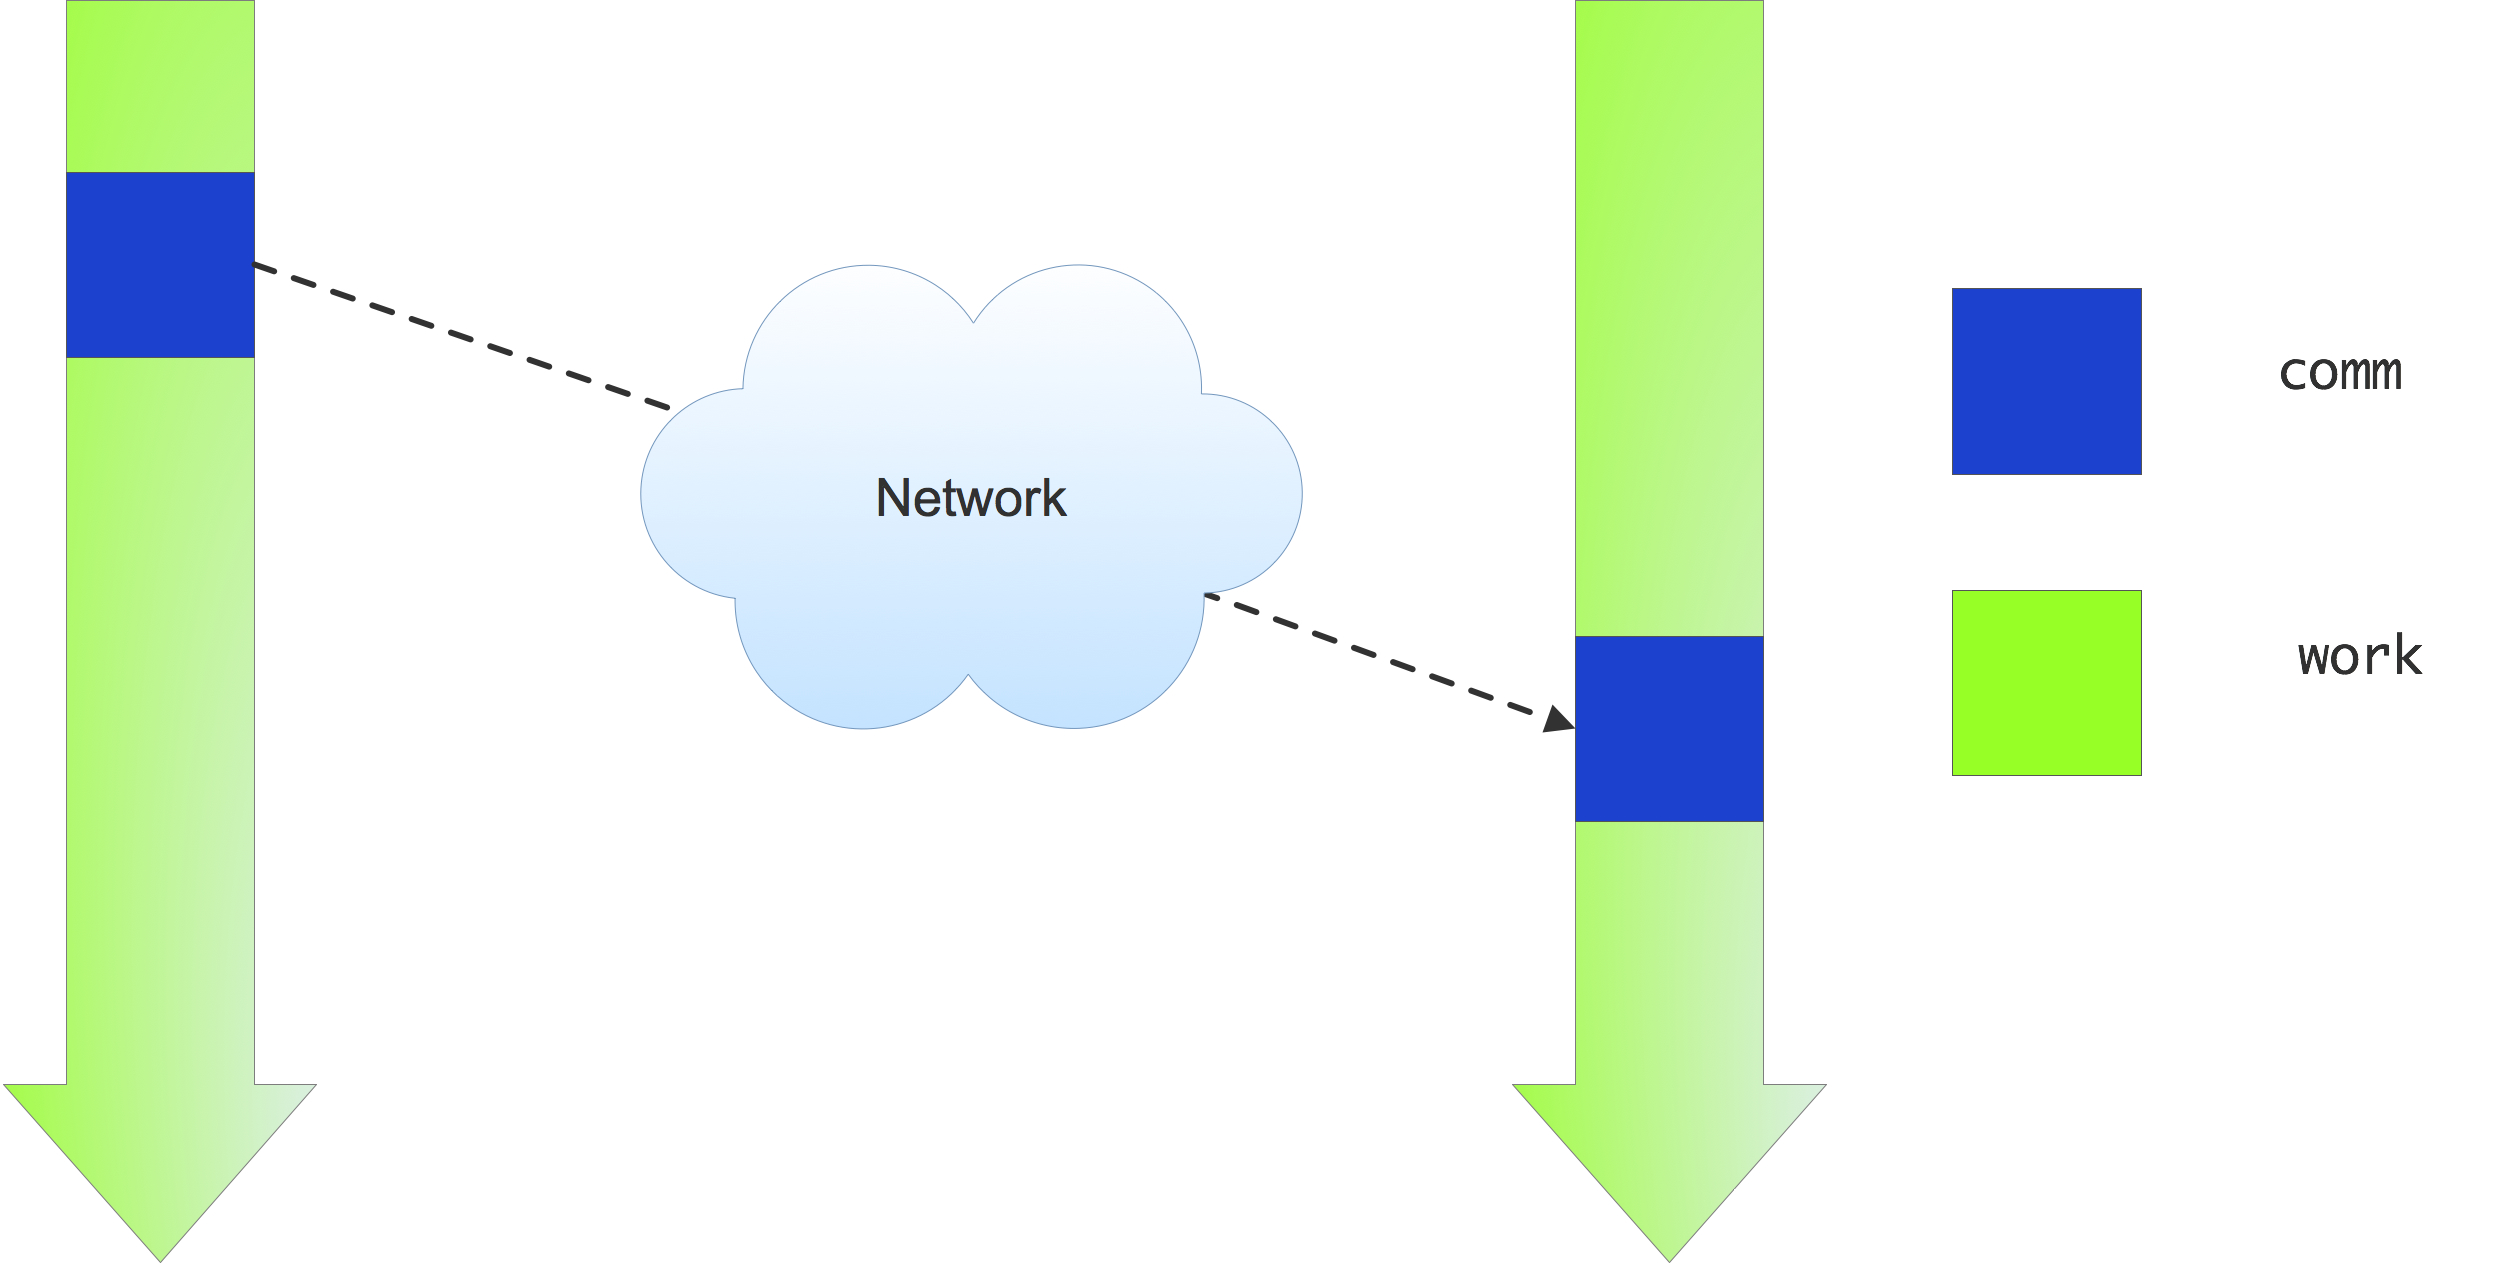
\includegraphics[scale=.1]{graphics-public/send-ideal}
\caption{Illustration of an ideal send-receive interaction}
\label{fig:send-ideal}
\end{figure}
Of course, if the receiving process gets to the receive call before
the send call has been issued, it will be idle until that happens.

Even if processes are optimally synchronized communication introduces
some overhead: there is an inital latency connected with every
message, and the network also has a limited bandwidth which leads to a
transfer time per byte; see~\HPSCref{sec:bwlatency}.

The above ideal scenario is not realistic: it assumes that somewhere
in the network there is buffer capacity for all messages that are in
transit. Since this message volume can be large, we have to worry
explicitly about management of send and receive \indexterm{buffers}.

The easiest scenario is that the sending process keeps the message
data in its address space until the receiving process has indicated
that it is ready to receive it. This is pictured in
figure~\ref{fig:send-blocking}.
\begin{figure}[ht]
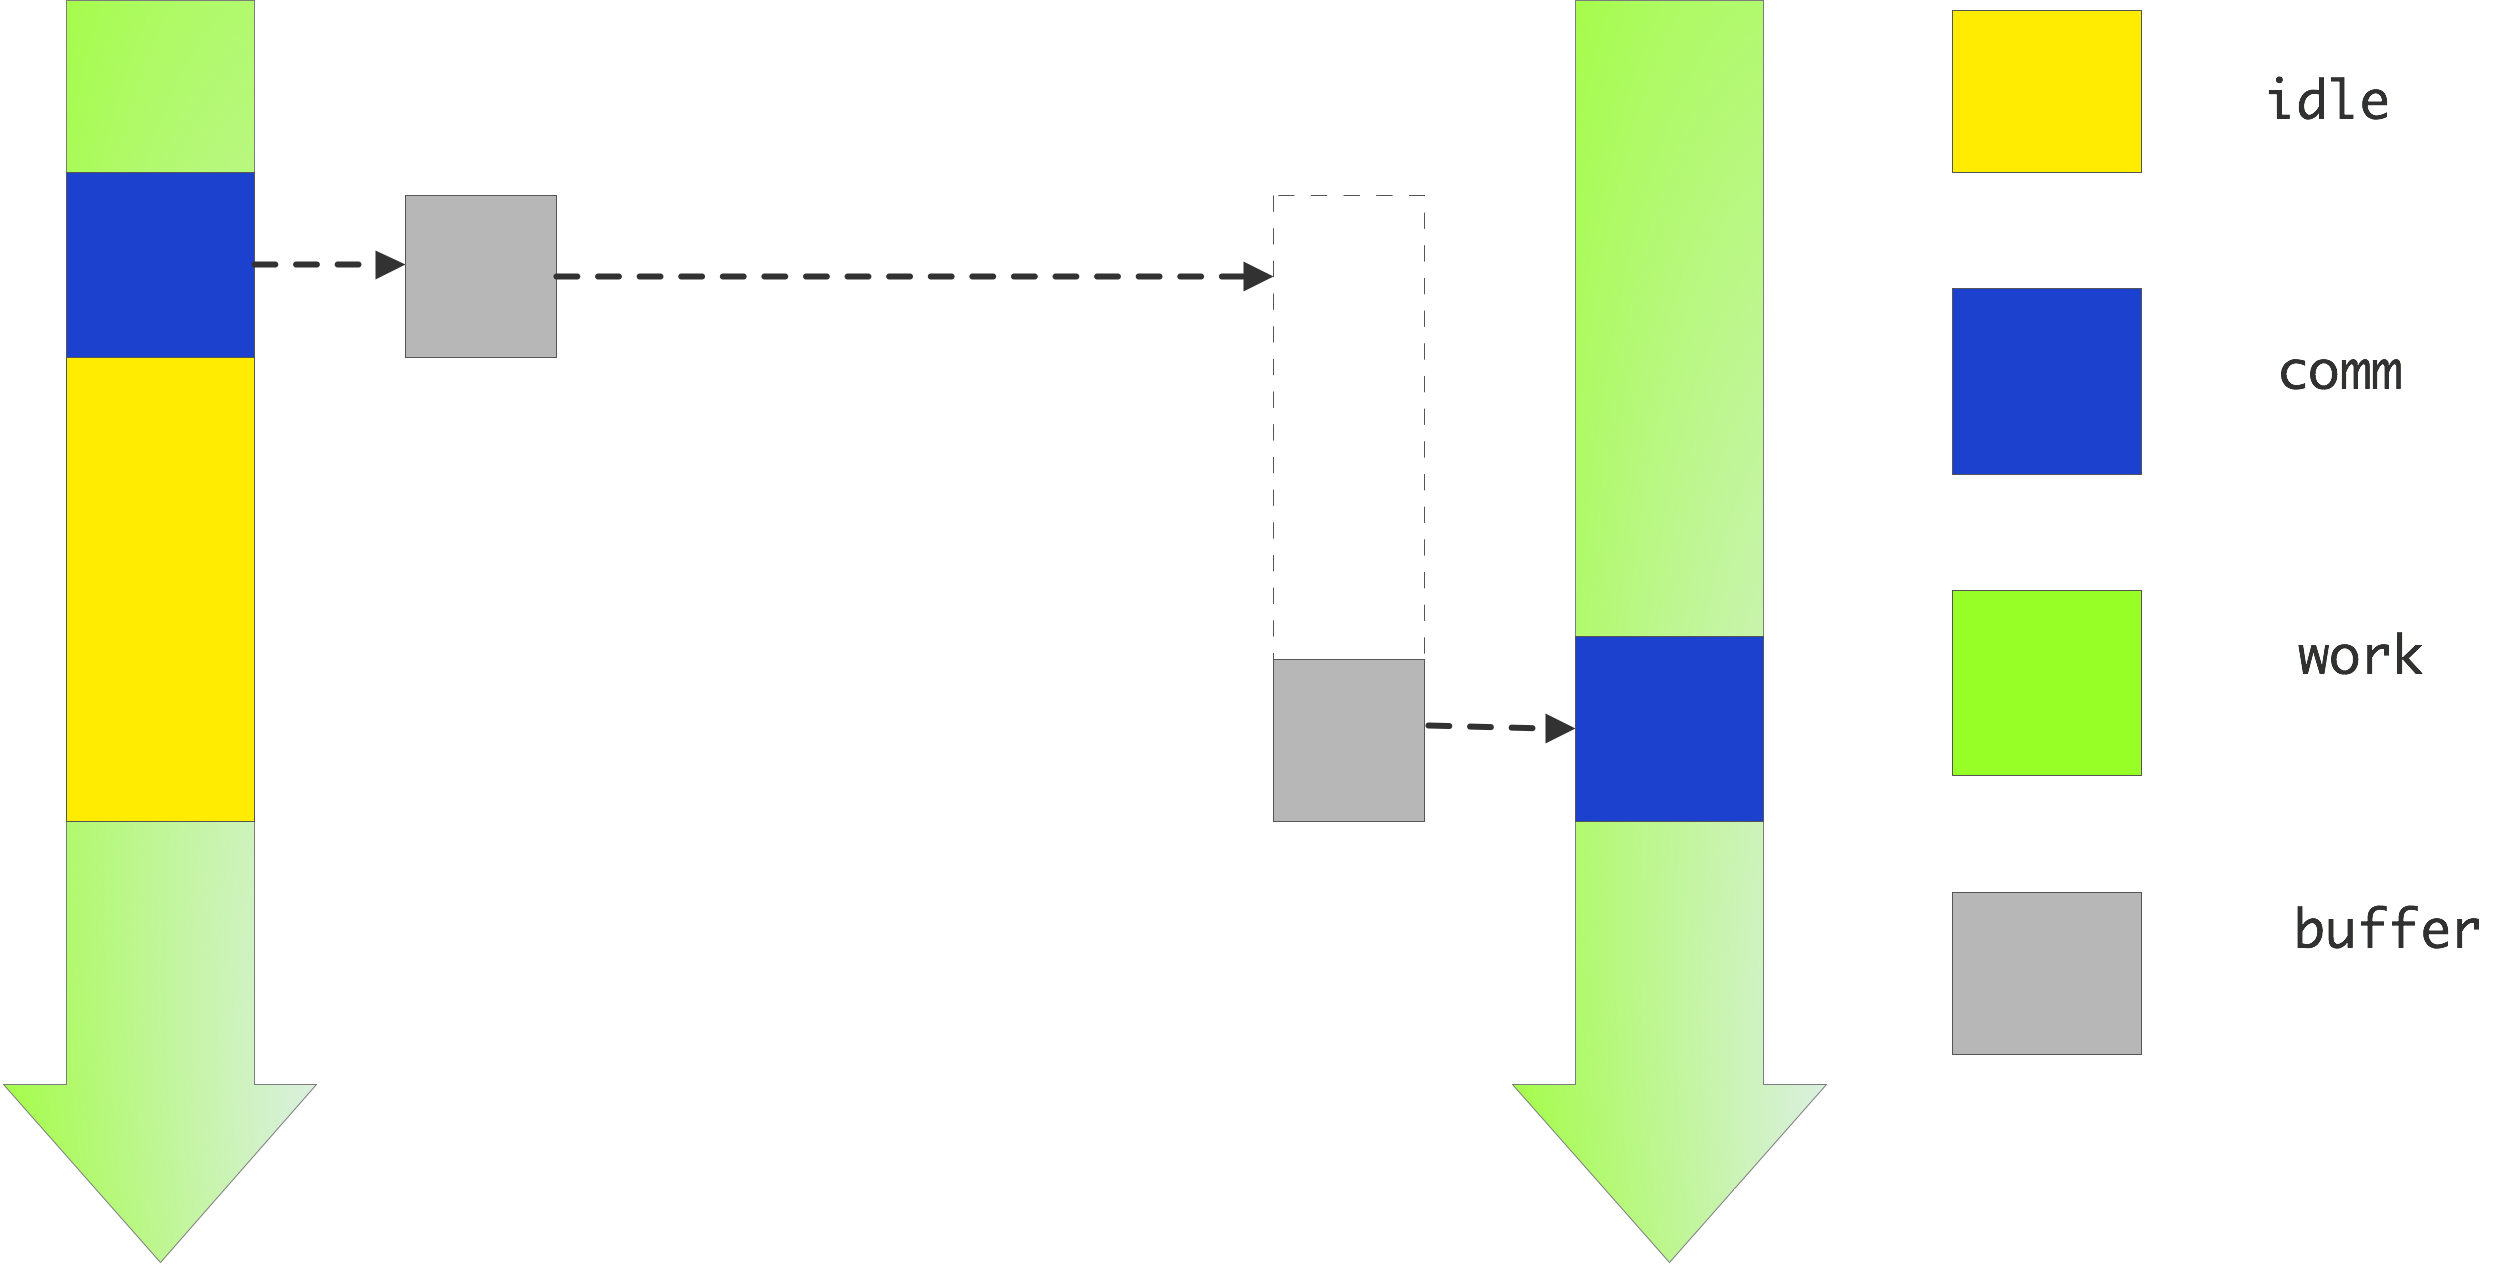
\includegraphics[scale=.1]{graphics-public/send-blocking}
\caption{Illustration of a blocking communication: the sending processor is idle until the receiving processor issues and finishes the receive call}
\label{fig:send-blocking}
\end{figure}
This is known as \emph{blocking} communication: a process that issues
a send or receive call will then block until the corresponding receive
or send call is successfully concluded.

It is clear what the first problem with this scenario is: if your
processes are not perfectly synchronized your performance may degrade
because processes spend time waiting for each other;
see~\HPSCref{sec:load}. 

But there is a more insidious, more serious problem.
Suppose two process need to exchange data, and consider the following
pseudo-code, which purports to exchange data between processes 0 and~1:
\begin{verbatim}
other = 1-mytid; /* if I am 0, other is 1; and vice versa */
send(target=other);
receive(source=other);
\end{verbatim}
Imagine that the two processes execute this code. They both issue the
send call\ldots\ and then can't go on, because they are both waiting
for the other to issue a receive call. This is known
as \indexterm{deadlock}.

The solution is to first do the send from 0 to~1, and then from 1 to~0 (or the other way around). So the code would look like:
\begin{verbatim}
if ( /* I am processor 0 */ ) {
  send(target=other);
  receive(source=other);
} else {
  receive(source=other);
  send(target=other);
}
\end{verbatim}

There is even a third, even more subtle problem with blocking
communication. Consider the scenario where every processor needs to
pass data to its successor, that is, the processor with the next
higher rank. The basic idea would be to first send to your successor,
then receive from your predecessor. Since the last processor does not
have a successor it skips the send, and likewise the first processor
skips the receive. The pseudo-code looks like:
\begin{verbatim}
successor = mytid+1; predecessor = mytid-1;
if ( /* I am not the last processor */ )
  send(target=successor);
if ( /* I am not the first processor */ )
  receive(source=predecessor)
\end{verbatim}
This code does not deadlock. All processors but the last one block on
the send call, but the last processor executes the receive call. Thus,
the processor before the last one can do its send, and subsequently
continue to its receive, which enables another send, et cetera.

In one way this code does what you intended to do:
it will terminate (instead of hanging forever on a
deadlock) and exchange data the right way. However, the execution
now suffers from \indextermsub{unexpected}{serialization}: only
one processor is active at any time, so what should have been a
\begin{figure}[ht]
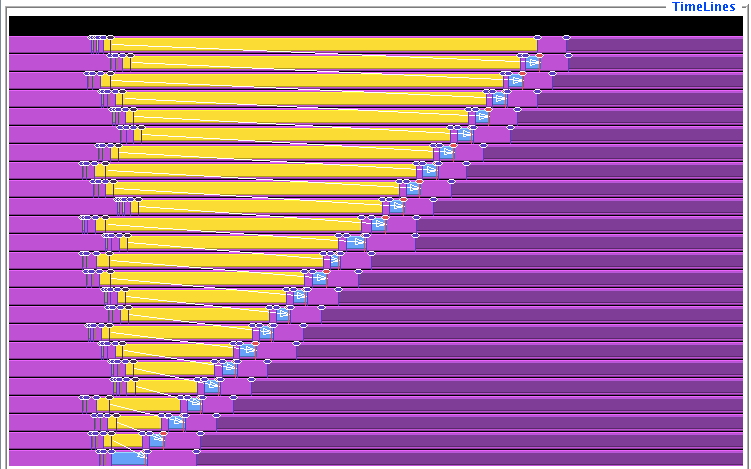
\includegraphics[scale=.4]{graphics-public/linear-serial}
\caption{Trace of a simple send-recv code}
\label{fig:serialization}
\end{figure}
parallel operation becomes a sequential one. This is illustrated in
figure~\ref{fig:serialization}.
\begin{exercise}
\label{ex:linear-sequential}
  Modify your earlier code, run it and reproduce the trace output 
  of figure~\ref{fig:serialization}.
\end{exercise}
It is possible to orchestrate your processes to get an efficient and
deadlock-free execution, but doing so is a bit cumbersome.
There are better solutions which we will
explore next.

\begin{exercise}
  Give pseudo-code for a solution that uses blocking operations, and is
  parallel, although maybe not optimally so.
\end{exercise}

\begin{exercise}
  There are rare circumstances where you actually want this serial
  behaviour. Recall from exercise~\ref{ex:hello-world-zero} that
  output from processes is not automatically serialized. Take your
  code from that exercise, and use the serialization behaviour your
  observed to force the processes to output their print statements in
  sequence.
\end{exercise}

Above, you saw a code fragment with a conditional send:
\begin{verbatim}
MPI_Comm_rank( .... &mytid );
successor = mytid+1
if ( /* I am not the last processor */ )
  send(target=successor);
\end{verbatim}
MPI allows for the following variant which makes the code slightly 
more homogeneous:
\begin{verbatim}
MPI_Comm_rank( .... &mytid );
if ( /* I am not the last processor */ )
  successor = mytid+1
else
  successor = MPI_PROC_NULL;
send(target=successor);
\end{verbatim}
where the send call is executed by all processors; the target value
of \indexmpishow{MPI_PROC_NULL} means that no actual send is done. 
The null processor
value is also of use with the \n{MPI_Sendrecv} call.

\Level 2 {Deadlock-free blocking communication}

Above you saw that with blocking sends the precise ordering of the
send and receive calls is crucial. Use the wrong ordering and you get
either deadlock, or something that is not efficient at all in
parallel. MPI has a way out of this problem that is sufficient for
many purposes: the combined send/recv call
\begin{verbatim}
MPI_Send_recv( /* send data */ ....
               /* recv data */ .... );
\end{verbatim}
This call makes it easy to exchange data between two processors: both
specify the other as both target and source. However, there need not
be any such relation between target and source: it is possible to
receive from a predecessor in some ordering, and send to a successor
in that ordering.

Above you saw some examples that had most processors doing both a send and
a receive, but some only a send or only a receive. You can still use
\n{MPI_Sendrecv} in this call if you use \n{MPI_PROC_NULL} for
the unused source or target argument.

\begin{exercise}
\label{ex:linear-sendrecv}
  Take your code from exercise~\ref{ex:linear-sequential}
  and rewrite it to use the \n{MPI_Sendrecv} call. Run it and
  produce a trace output. Do you see the serialization behaviour
  of your earlier code?
\end{exercise}


\Level 2 {Subtleties with processor synchronization}
\label{sec:handshake}

Blocking communication involves a complicated dialog between the two
processors involved. Processor one says `I~have this much data to
send; do you have space for that?', to which processor two replies
`yes, I~do; go ahead and send', upon which processor one does the
actual send. This back-and-forth (technically known as
a \indexterm{handshake}) takes a certain amount of communication
overhead. For this reason, network hardware will sometimes forgo the
handshake for small messages, and just send them regardless, knowing
that the other process has a small buffer for such occasions.

%This behaviour is not dictated by the standard: it is up to the implementation
%to make this optimization for small messages.

One strange side-effect of this strategy is that a code that
should \indexterm{deadlock} according to the MPI specification does
not do so. In effect, you may be shielded from you own programming
mistake! Of course, if you then run a larger problem, and the small
message becomes larger than the threshold, the deadlock will suddenly
occur. So you find yourself in the situation that a bug only manifests
itself on large problems, which are usually harder to debug. In this
case, replacing every \n{MPI_Send} with a \indexmpishow{MPI_Ssend} will force the
handshake, even for small messages.

Conversely, you may sometimes wish to avoid the handshake on large
messages. MPI as a solution for this: the \indexmpishow{MPI_Rsend} (`ready
send') routine sends its data immediately, but it needs the receiver
to be ready for this. How can you guarantee that the receiving process
is ready? You could for instance do the following (this uses
non-blocking routines, which are explained below in
section~\ref{sec:nonblocking}):
\begin{verbatim}
if ( receiving ) {
  MPI_Irecv()   // post non-blocking receive
  MPI_Barrier() // synchronize
else if ( sending ) {
  MPI_Barrier() // synchronize
  MPI_Rsend()   // send data fast
\end{verbatim}
When the barrier is reached, the receive has been posted, so it is safe 
to do a ready send. However, global barriers are not a good idea.
Instead you would just synchronize the two processes involved.
\begin{exercise}
  Give pseudo-code for a scheme where you synchronize the two
  processes through the exchange of a blocking zero-size message.
\end{exercise}

\index{communication!blocking|)}

\Level 1 {Non-blocking communication}
\commandref{sec:nonblocking}
\index{communication!non-blocking|(}

In the previous section you saw that blocking communication makes
programming tricky if you want to avoid deadlock and performance
problems. The main advantage of these routines is that you have full
control about where the data is.  By contrast, \emph{non-blocking}
communication routines are easier to use, but more wasteful of memory.

The non-blocking calls \indexmpishow{MPI_Isend} and \indexmpishow{MPI_Irecv}
do not wait for their counterpart: in effect they tell the runtime
system `here is some data and please send it as follows' or `here is
some buffer space, and expect such-and-such data to
come'. 
This is illustrated in figure~\ref{fig:send-nonblocking}.

While the use of non-blocking routines prevents deadlock, it
introduces two new problems:
\begin{enumerate}
\item When the send call returns, the send buffer may not be safe to
  overwrite; when the recv call returns, you do not know for sure that
  the expected data is in it. Thus, you need a mechanism to make sure
  that data was actually sent or received.
\item With a blocking send call, you could repeatedly fill the send
  buffer and send it off. To send multiple messages with non-blocking calls
  you have to allocate multiple buffers.
\end{enumerate}

For the first problem, MPI has two types of
routines. The \indexmpishow{MPI_Wait...} calls are blocking: when you issue
such a call, your execution will wait until the specified requests
have been completed. A~typical way of using them is:
\begin{verbatim}
// start non-blocking communication
MPI_Isend( ... ); MPI_Irecv( ... );
// do work that does not depend on incoming data
....
// wait for the Isend/Irecv calls to finish
MPI_Wait( ... );
// now do the work that absolutely needs the incoming data
....
\end{verbatim}
There are several wait calls:
\begin{itemize}
\item \indexmpishow{MPI_Wait} waits for a a single request. If you are
  indeed waiting for a single nonblocking communication to complete,
  this is the right routine. If you are waiting for multiple requests
  you could call this routine in a loop. 
\begin{verbatim}
for (p=0; p<nrequests ; p++)
  MPI_Wait(request[p],&(status[p]));
\end{verbatim}
  However, this would be inefficient if the first request is fulfilled much later than 
  the others: your waiting process would have lots of idle time. In that case,
  use one of the following routines.
\item \indexmpishow{MPI_Waitall} allows you to wait for a number of
  requests, and it does not matter in what sequence they are
  satisfied. Using this routine is easier to code than the loop above,
  and it could be more efficient.
\item The `waitall' routine is good if you have need all nonblocking
  communications to be finished before you can proceed with the rest
  of the program. However, sometimes it is possible to take action as
  each request is satisfied. In that case you could use
  \indexmpishow{MPI_Waitany} and write:
\begin{verbatim}
for (p=0; p<nrequests; p++) {
  MPI_Waitany(nrequests,request_array,&index,statuses);
  // operate on buffer[index]
}
\end{verbatim}
\item \indexmpishow{MPI_Waitsome} is very much like \n{Waitany},
  except that it returns multiple numbers, if multiple requests are
  satisfied.
\end{itemize}

Figure~\ref{fig:jump-nonblock} shows the trace of a non-blocking execution
using \n{MPI_Waitall}.
\begin{figure}[ht]
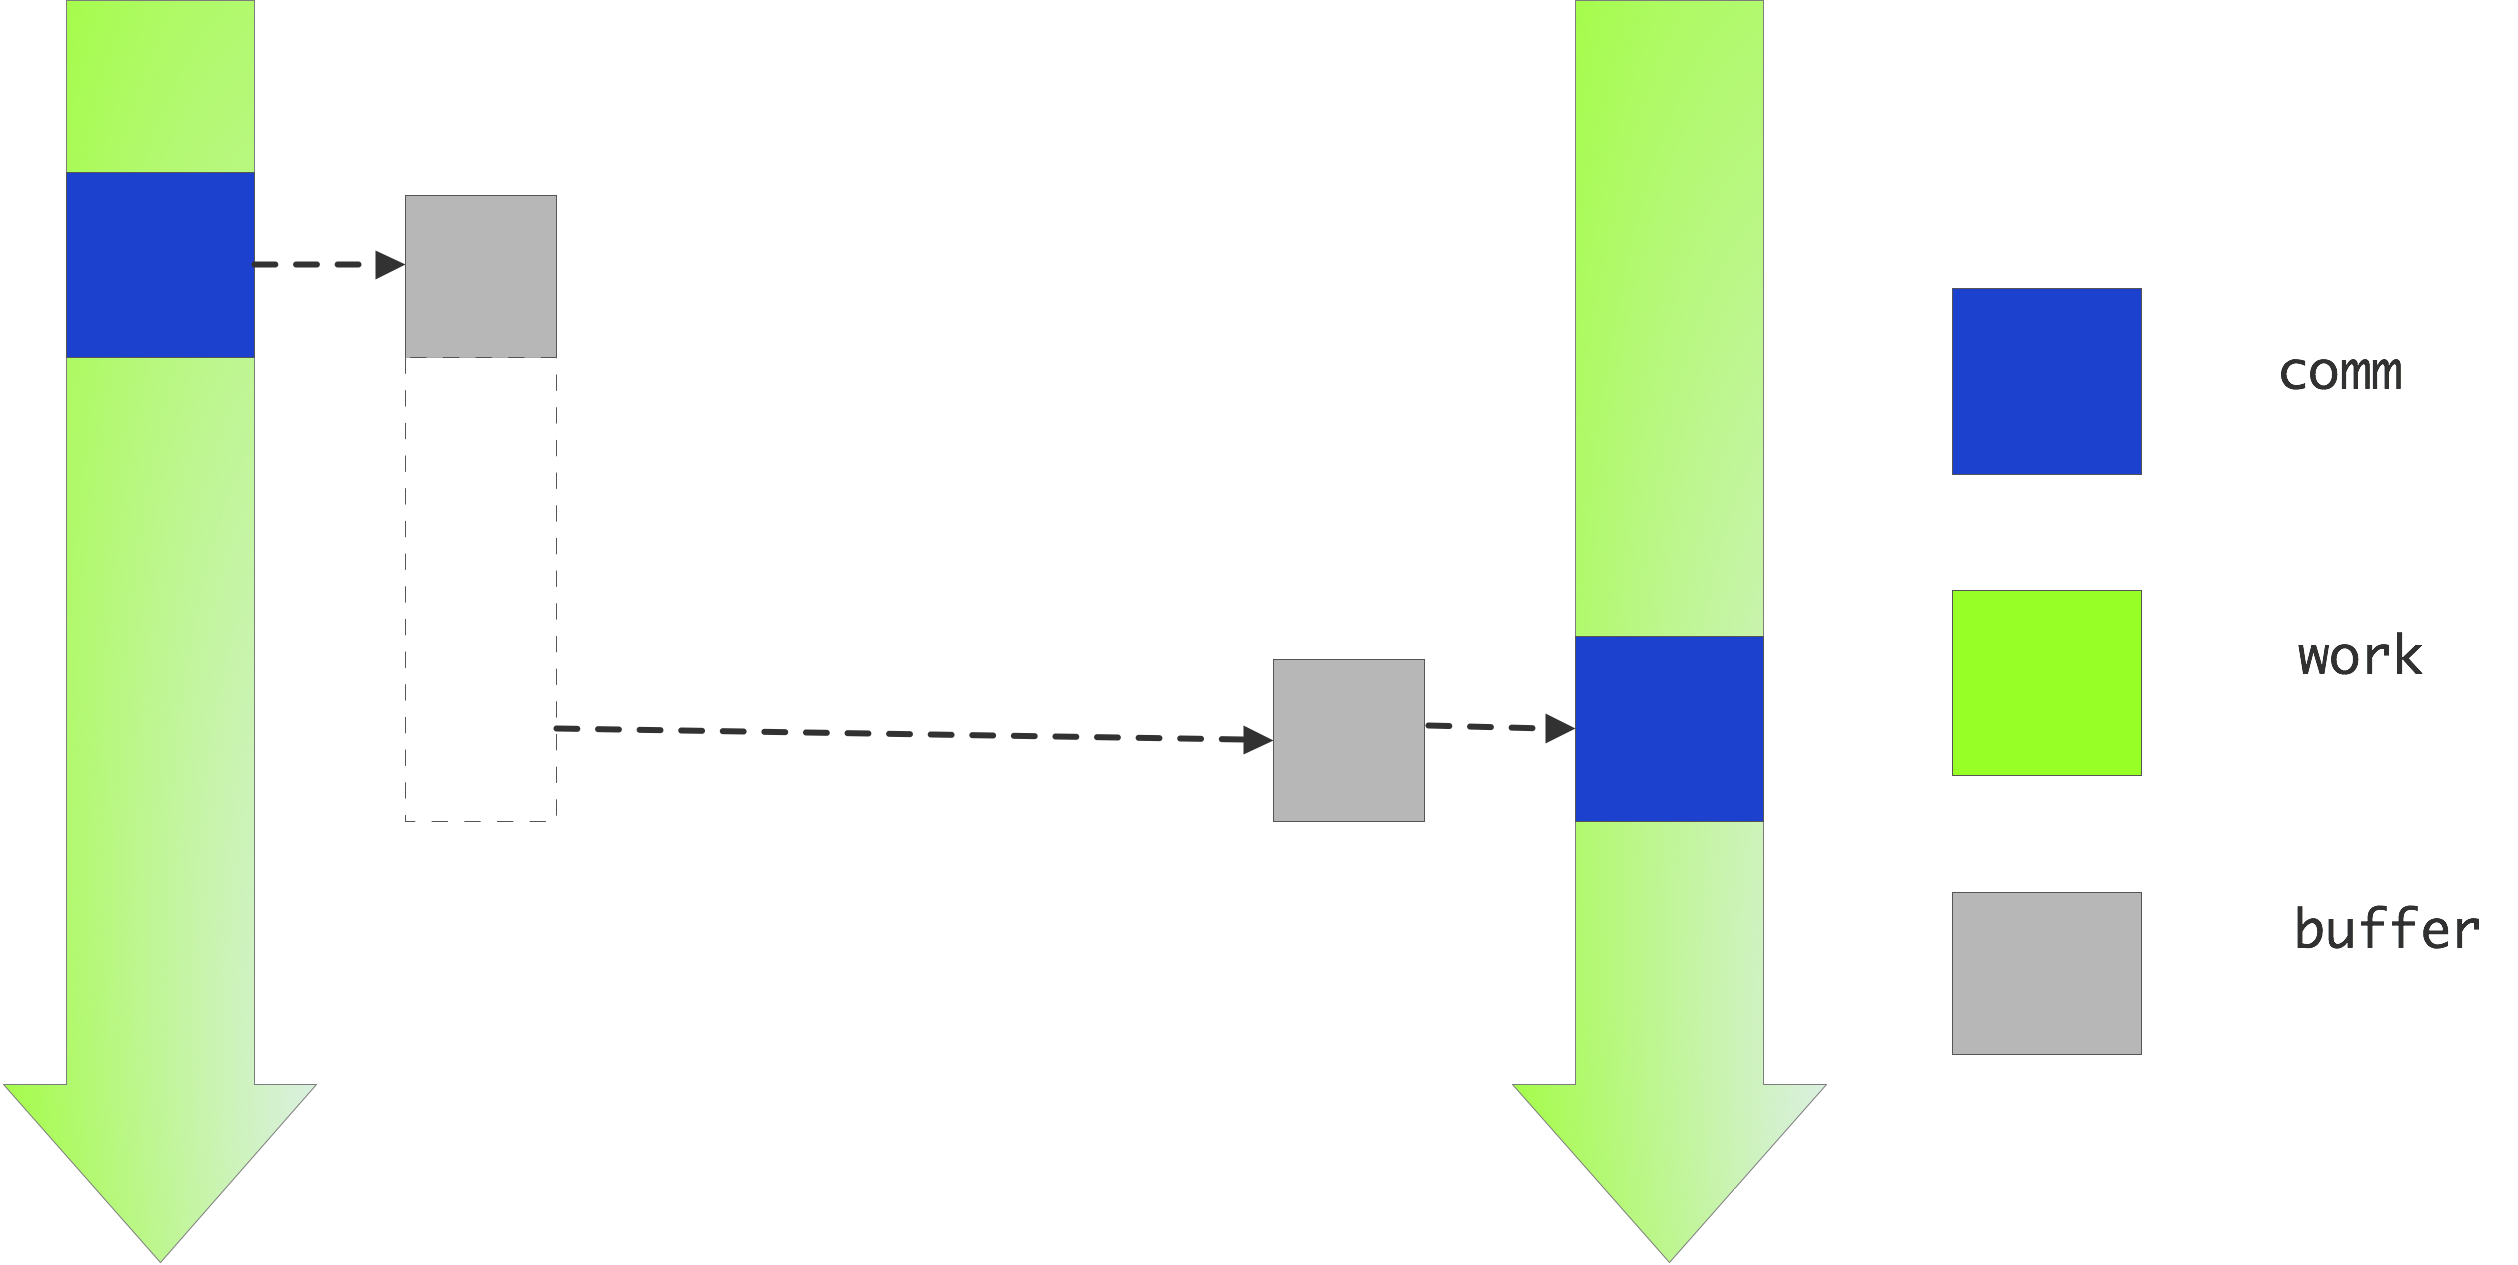
\includegraphics[scale=.1]{graphics-public/send-nonblocking}
\caption{Illustration of a non-blocking communication: the sending processor immediately continues execution after issueing the send call}
\label{fig:send-nonblocking}
\end{figure}
\begin{figure}[ht]
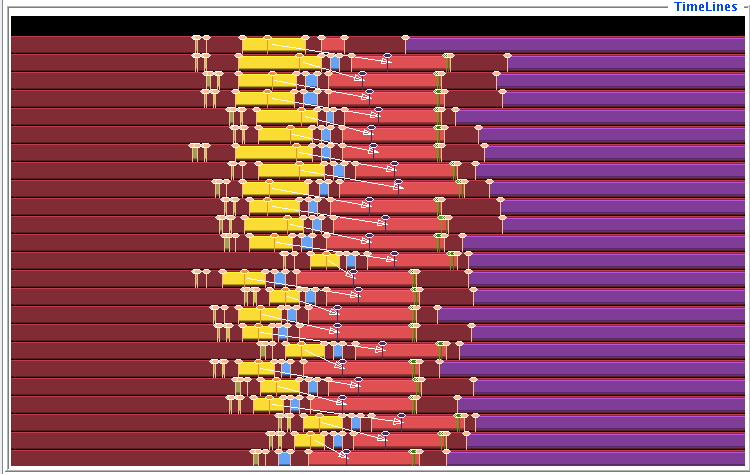
\includegraphics[scale=.4]{graphics-public/linear-nonblock}
\caption{A trace of a nonblocking send between neighbouring processors}
\label{fig:jump-nonblock}
\end{figure}

The \n{MPI_Test....} calls are themselves non-blocking: they
test for whether one or more requests have been
fullfilled. Here a typical idiom would be:
\begin{verbatim}
// start non-blocking communication
for ( ... p ... ) {
  MPI_Isend( .. p .. ); MPI_Irecv( .. p .. );
}
// wait for incoming data and process
while ( .. there are still requests .. ) {
  MPI_Test( ... );
  p = message.source;
  // process data from p
}
\end{verbatim}

\begin{exercise}
  Read section~\HPSCref{sec:pspmvp} and give pseudo-code for the
    distributed sparse matrix-vector product using the above idiom for
    using \n{MPI_Test...} calls. Discuss the advantages and
    disadvantages of this approach. The answer is not going to be
    black and white: discuss when you expect which approach to be
    preferable.
\end{exercise}

Another scenario where \n{MPI_Wait} calls are convenient is in the
\indexterm{master-worker model}. The master process creates tasks, and
sends them to whichever worker process has finished its work:
\begin{verbatim}
while ( not done ) {
  // create new inputs for a while
  ....
  // see if anyone has finished
  MPI_Test( .... &index, &flag );
  if ( flag ) {
    // receive processed data and send new
}
\end{verbatim}

\Level 2 {Overlap of computation and communication}

Non-blocking routines have long held the promise of letting a
program \emph{overlap its computation and
communication}\index{communication!overlap with computation}.  The
idea was that after posting the non-blocking calls the program could
proceed to do non-communication work, while another part of the system
would take care of the communication. Unfortunately, a~lot of this 
communication involved activity in user space, so the solution would have
been to let it be handled by a separate thread. Until recently, processors
were not efficient at doing such multi-threading, so true overlap 
stayed a promise for the future.

\Level 2 {More about non-blocking}

Above we used \n{MPI_Irecv}, but we could have used the \n{MPI_Recv}
routine.  There is nothing special about a non-blocking or synchronous
message once it arrives; the \n{MPI_Recv} call can match any of the
send routines you have seen so far (but not \n{MPI_Sendrecv}).

% MPI_Cancel( &request )

% MPI_Probe

\index{communication!non-blocking|)}
\index{communication!two-sided|)}
\Level 1 {One-sided communication}
\commandref{sec:one-sided}
\index{communication!one-sided|(}
\index{target!active synchronization|see{active target synchronization}}
\index{target!passive synchronization|see{passive target synchronization}}

Above, you saw collectives and point-to-point operations. The latter
type had in common that they require the co-operation of a sender and
receiver. This co-operation could be loose: you can post a receive
with \n{MPI_ANY_SOURCE} as sender, but there had to be both a send and
receive call. On the other hand, in one-sided communication a process
can do a `put' or `get' operation, writing data to or reading it from
another processor, without that other processor's involvement.

In one-sided MPI operations, also known as \acf{RDMA} or 
\acf{RMA} operations, there
are still two processes involved: the \indexterm{origin}, which is the
process that originates the transfer, whether this is a `put' or a `get',
and the \indexterm{target} whose
memory is being accessed. On the target, you declare an area of
user-space memory that is accessible to other processes. This is known
as a \indexterm{window}. Windows limit how origin processes can access
the target's memory: you can only `get' data from a window or `put' it
into a window; all the other memory is not reachable from other processes.

The alternative to having windows is to use \indexterm{distributed shared memory}
or \indexterm{virtual shared memory}: memory is distributed but acts as if
it shared. The so-called \acf{PGAS} languages such as \ac{UPC} use this model.
The MPI \ac{RMA} model makes it possible to 
lock a window which makes programming slightly more cumbersome, but the
implementation more efficient.

Within one-sided communication, MPI has two modes: active RMA and
passive RMA. In \indextermsub{active}{RMA}, or \indexterm{active target synchronization},
both parties are involved; the main advantage
of this mode is that the origin program can perform many small transfers, which are
aggregated behind the scenes. Active RMA acts much like asynchronous transfer with a
concluding \n{Waitall}.

In \indextermsub{passive}{RMA}, or \indexterm{passive target synchronization},
the target process is not involved. 
(\ac{PGAS} languages such as \ac{UPC} are based on this model: data is 
simply read or written at will.)
While 
intuitively it is attractive to be able to write to and read from arbitrary memory,
there are practical problems. For instance, it requires a remote agent on the target,
which may interfere with execution of the main thread, or conversely it may not be
activated at the optimal time. Passive RMA is also very hard to debug and can lead
to strange deadlocks.

%% McLaren says use an info object

\Level 2 {Windows}
\commandref{sec:windows}
\index{window|(}

A window is a contiguous area of memory,
\begin{figure}[ht]
  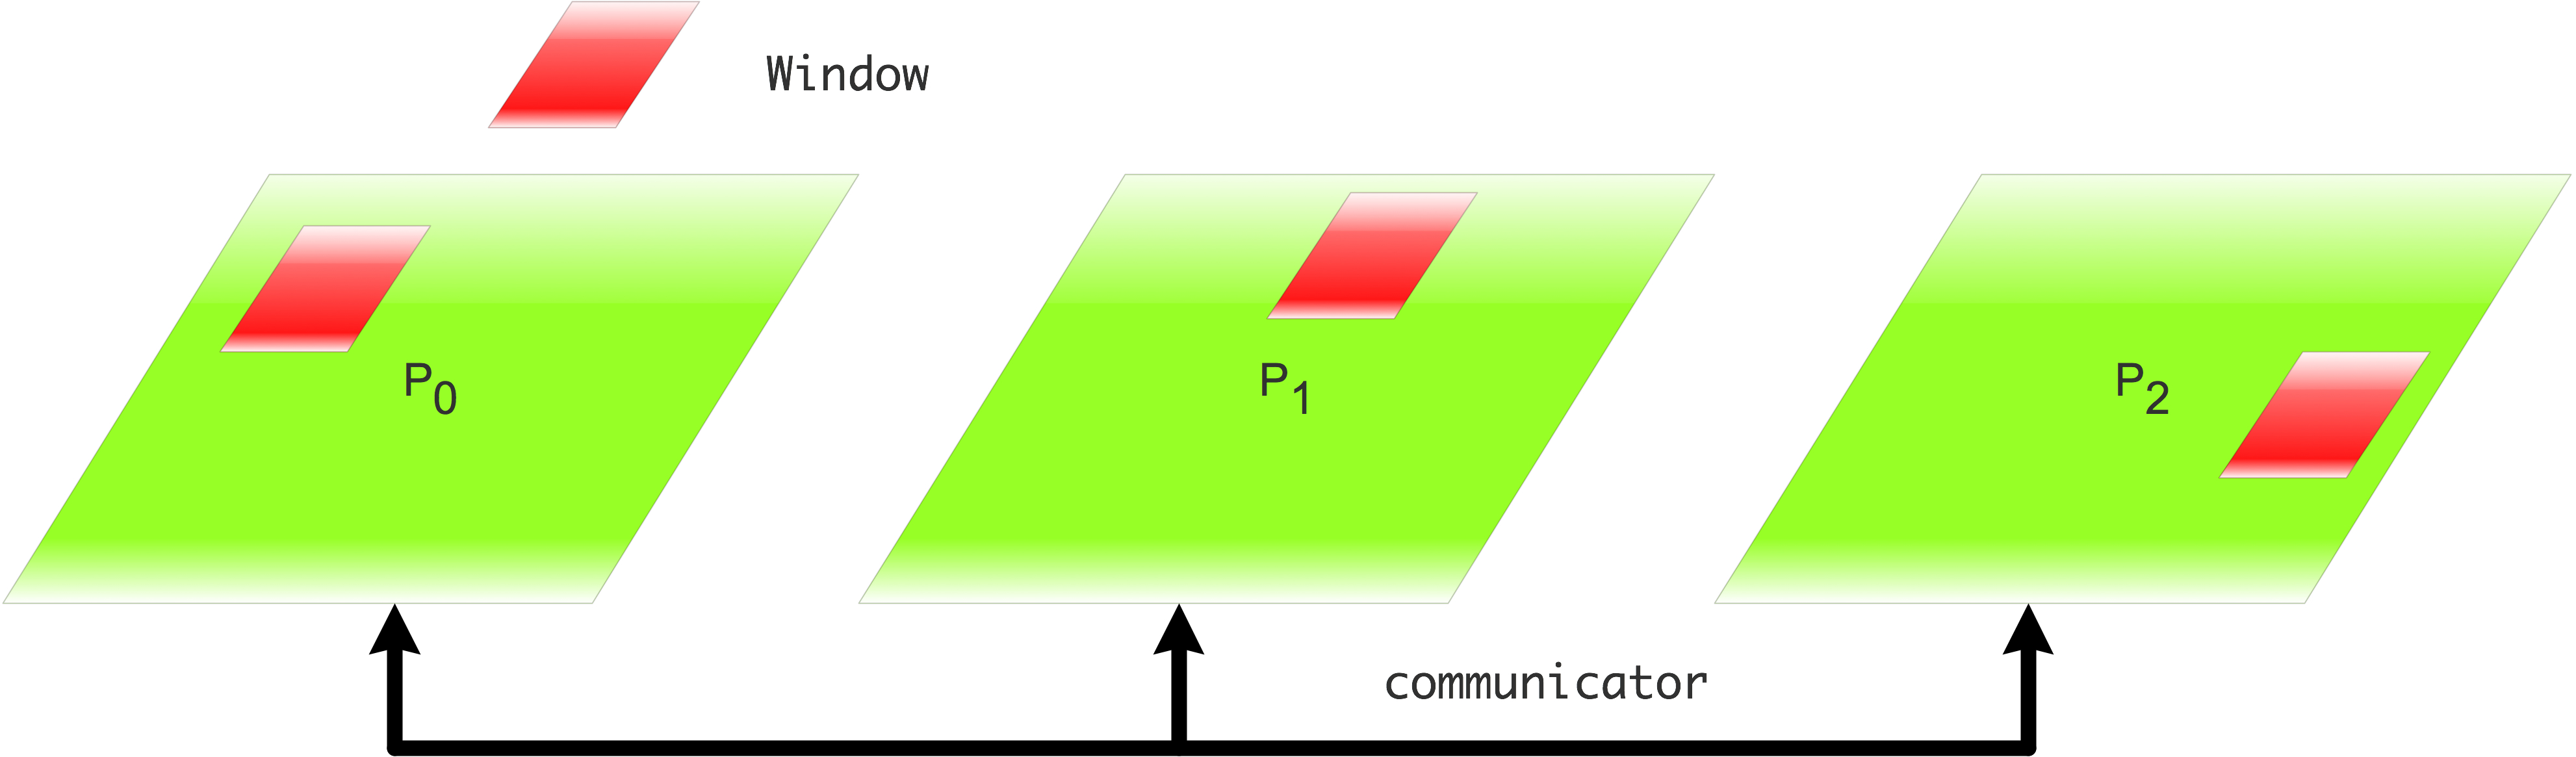
\includegraphics[scale=.1]{graphics-public/one-sided-window}
  \caption{Collective definition of a window for one-sided data access}
  \label{fig:window}
\end{figure}
defined with respect to a communicator: each process specifies a
memory area. Routine for creating and releasing windows
are collective, so each process \emph{has} to
call them; see figure~\ref{fig:window}. 
\begin{verbatim}
MPI_Info info;
MPI_Win window;
MPI_Win_create( /* size */, info, comm, &window );
MPI_Win_free( &window );
\end{verbatim}
(For the \n{info} parameter you can often use \indexmpishow{MPI_INFO_NULL}.)
While the creation of a window is collective, each
processor can specify its own window size, including zero, and even the type of the
elements in it.

\Level 2 {Active target synchronization: epochs}

There are two mechanisms for \indexterm{active target synchronization}, that is,
one-sided communications where both sides are involved to the extent that they declare
the communication epoch. In this section we look at the first mechanism,
which is to use a \indexterm{fence} operation:\indexmpi{MPI_Win_fence}
\begin{verbatim}
MPI_Win_fence (int assert, MPI_Win win, ierr)
\end{verbatim}
This operation is collective on the communicator of the window.
It is comparable to \n{MPI_Wait} calls for non-blocking communication.

Unlike with wait calls, you always need two fences: one before and one after
the so-called \indexterm{epoch}. 
You can give various hints to the system about this epoch versus the ones
before and after through the \n{assert} parameter.
\begin{verbatim}
MPI_Win_fence((MPI_MODE_NOPUT | MPI_MODE_NOPRECEDE), win);
MPI_Get( /* operands */, win);
MPI_Win_fence(MPI_MODE_NOSUCCEED, win);
\end{verbatim}
In between the two fences the window is exposed, and while it is you
should not access it locally. If you absolutely need to access it
locally, you can use an \ac{RMA} operation for that. Also, there can be only one
remote process that does a \n{put}; multiple \n{accumulate} accesses are allowed.

Fences are, together with other window calls, collective operations. That means they 
imply some amount of synchronization between processes. Consider:
\begin{verbatim}
MPI_Win_fence( ... win ... ); // start an epoch
if (mytid==0) // do lots of work
else // do almost nothing
MPI_Win_fence( ... win ... ); // end the epoch
\end{verbatim}
and assume that all processes execute the first fence more or less at the same time.
The zero process does work before it can do the second fence call, but all other
processes can call it immediately. However, they can not finish that second fence call
until all one-sided communication is finished, which means they wait for the zero process.
\begin{figure}[ht]
  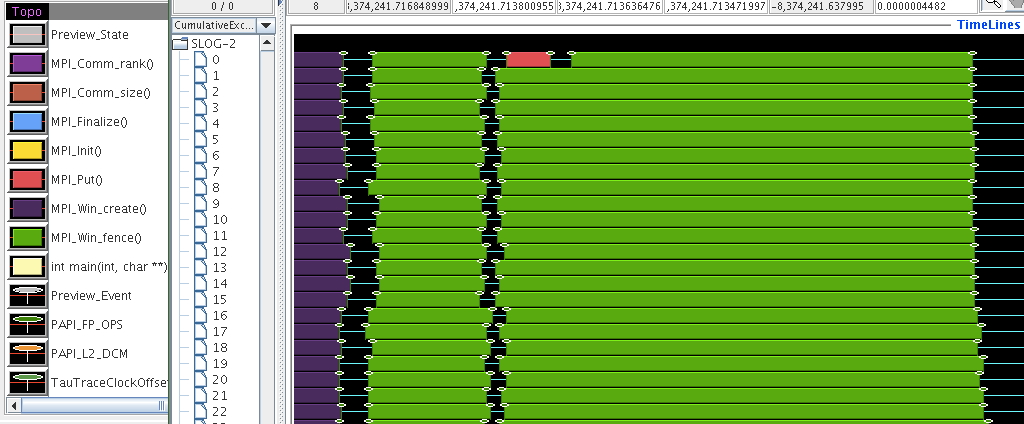
\includegraphics[scale=.4]{graphics-public/putblock}
  \caption{A trace of a one-sided communication epoch where process zero only originates
  a one-sided transfer}
  \label{fig:putblock}
\end{figure}

As a further restriction, you can not mix \n{Get} with \n{Put} or \n{Accumulate}
calls in a single epoch. Hence, we can characterize an epoch as an
\indextermsub{access}{epoch} on the origin, and
as an \indextermsub{exposure}{epoch} on the target.

Assertions are an integer parameter: you can add or logical-or values.
The value zero is always correct. There are two types of parameters.
Local assertions are:
\begin{itemize}
  \item\indexmpishow{MPI_MODE_NOSTORE} The preceding epoch did not store
    anything in this window.
  \item\indexmpishow{MPI_MODE_NOPUT} The following epoch will not store
    anything in this window.
\end{itemize}
Global assertions:
\begin{itemize}
  \item\indexmpishow{MPI_MODE_NOPRECEDE} This process made no \ac{RMA}
    calls in the preceding epoch.  
  \item\indexmpishow{MPI_MODE_NOSUCCEED} This process will make no
    \ac{RMA} calls in the next epoch.
\end{itemize}


\index{window|)}

\Level 2 {Put, get, accumulate}

Window areas are 
accessible to other processes in the communicator by specifying the
process rank and an offset from the base of the window.
\begin{verbatim}
MPI_Put (
  void *origin_addr, int origin_count, MPI_Datatype origin_datatype,
  int target_rank,
  MPI_Aint target_disp, int target_count, MPI_Datatype target_datatype,
  MPI_Win window)
\end{verbatim}
The \n{MPI_Get} call is very similar; a third one-sided routine
is \n{MPI_Accumulate} which does a reduction operation on the results
that are being put:
\begin{verbatim}
MPI_Accumulate (
  void *origin_addr, int origin_count, MPI_Datatype origin_datatype, 
  int target_rank,
  MPI_Aint target_disp, int target_count, MPI_Datatype target_datatype,
  MPI_Op op,MPI_Win window)
\end{verbatim}

\begin{exercise}
  Implement an `all-gather' operation using one-sided communication:
  each processor stores a single number, and you want each processor
  to build up an array that contains the values from all
  processors. Note that you do not need a special case for a processor
  collecting its own value: doing `communication' between a processor
  and itself is perfectly legal.
\end{exercise}

Accumulate is a reduction with remote result. As with reduction, the 
order is undefined. The same predefined operators are available, but no
user-defined ones. One extra: \indexmpishow{MPI_REPLACE}.

\Level 2 {Put vs Get}

\begin{verbatim}
while(!converged(A)){ 
  update(A); 
  MPI_Win_fence(MPI_MODE_NOPRECEDE, win); 
  for(i=0; i < toneighbors; i++) 
    MPI_Put(&frombuf[i], 1, fromtype[i], toneighbor[i], 
                         todisp[i], 1, totype[i], win); 
  MPI_Win_fence((MPI_MODE_NOSTORE | MPI_MODE_NOSUCCEED), win); 
  } 
\end{verbatim}
\begin{verbatim}
  while(!converged(A)){ 
  update_boundary(A); 
  MPI_Win_fence((MPI_MODE_NOPUT | MPI_MODE_NOPRECEDE), win); 
  for(i=0; i < fromneighbors; i++) 
    MPI_Get(&tobuf[i], 1, totype[i], fromneighbor[i], 
                    fromdisp[i], 1, fromtype[i], win); 
  update_core(A); 
  MPI_Win_fence(MPI_MODE_NOSUCCEED, win); 
  } 
\end{verbatim}

\Level 2 {More active target synchronization}

There is a more fine-grained ways of doing 
\indexterm{active target synchronization}. While fences
corresponded to a global synchronization of one-sided calls,
the \n{MPI_Win_start},
\n{MPI_Win_complete}, \n{MPI_ Win_post}, \n{Win_wait} routines
are suitable, and possibly more efficient,
if only a small number of processor pairs is
involved.  Which routines
you use depends on whether the processor is an \indexterm{origin} or
\indexterm{target}.

If the current process is going to have the data in its window accessed,
you define an \indextermsub{exposure}{epoch} by:
\begin{verbatim}
MPI_Win_post( /* group of origin processes */ )
MPI_Win_wait()
\end{verbatim}
This turns the current processor into a target for access operations issued
by a different process.

If the current process is going to be issuing one-sided operations,
you define an \indextermsub{access}{epoch} by:
\begin{verbatim}
MPI_Win_start()
MPI_Win_complete()
\end{verbatim}
This turns the current process into the origin of a number of
one-sided access operations.

The `post' and `start' routines open the window to a
\indextermbus{group of}{processors}; see section~\ref{sec:comm-group}
for how to get such a group from a communicator.

\Level 2 {Passive target synchronization}

In \indexterm{passive target synchronization} only one processor
is involved in the communication. This involves using
a lock: one process can lock the window
on another, specified, process.
\begin{verbatim}
MPI_Win_lock (int locktype, int rank, int assert, MPI_Win win)
MPI_Win_unlock (int rank, MPI_Win win)
\end{verbatim}
During an access epoch, a process can initiate and finish a one-sided
transfer.
\begin{verbatim}
If (rank == 0) {
  MPI_Win_lock (MPI_LOCK_SHARED, 1, 0, win);
  MPI_Put (outbuf, n, MPI_INT, 1, 0, n, MPI_INT, win);
  MPI_Win_unlock (1, win);
}
\end{verbatim}
The two lock types are:
\begin{itemize}
\item \indexmpishow{MPI_LOCK_SHARED} which should be used for \n{Get}
  calls: since multiple processors are allowed to read from a window
  in the same epoch, the lock can be shared.
\item \indexmpishow{MPI_LOCK_EXCLUSIVE} which should be used for
  \n{Put} and \n{Accumulate} calls: since only one processor is
  allowed to write to a window during one epoch, the lock should be
  exclusive.
\end{itemize}
These routines make MPI behave like a shared memory system; the
instructions between locking and unlocking the window effectively
become \indexterm{atomic operations}.

\Level 2 {Details}

Sometimes an architecture has memory that is shared between processes,
or that otherwise is fast for one-sided communication. To put a window
in such memory, it can be placed in memory that is especially
allocated:
\begin{verbatim}
MPI_Alloc_mem() and MPI_Free_mem()
\end{verbatim}
These calls reduce to \n{malloc} and \n{free} is there is no special
memory area.

\index{communication!one-sided|)}

\Level 0 {Collectives}
\index{collectives|(}
\commandref{sec:collective}

Collectives are operations that involve all processes in a
communicator. The simplest example is a broadcast: one processor has
some data and all others need to get a copy of it.  A~collective is a
single call, and it blocks on all processors. That does not mean that
all processors exit the call at the same time: because of network
latency some processors can receive their data later than others.

The collective operations discussed in this section are:
\begin{itemize}
\item Broadcast, reduce, and scan: in these operations a single data
  item is sent from or collected on a `root' process.
\item Gather and scatter: here the root has an array from which to
  send, or in which to collect, the data from the other processors.
\item All-to-all, which lets all processors communicate with all others.
\item Barrier, which synchronizes all processes, and which separates
  events before it from those after it.
\end{itemize}
There are several variants of most collectives. For instance, the
gather and reduce calls have
a \indextermsub{root of the}{collective} where
information is collected.  There is a corresponding `all' variant,
where the result is not left just on the root but everywhere. 
There are also `v' variants where the
amount of data coming from or going to each processor is variable.

In addition to these collective operations, there are operations that
are said to be `collective on their communicator', but which do not
involve data movement. Collective then means that all processors must
call this routine; not to do so is an error that will probably
manifest itself in `hanging' code. One such example is
\n{MPI_Win_fence}.

\Level 1 {Broadcast, reduce, scan}
\label{sec:bcast}

The simplest collective is the broadcast, where one process has some
data that needs to be shared with all others. One scenario is that
processor zero can parse the commandline arguments of the executable.
The call has the following structure:
\begin{verbatim}
MPI_Bcast( data..., root , comm);
\end{verbatim}
The root is the process that is sending its data; see figure~\ref{fig:bcast-simple}.
\begin{figure}[ht]
  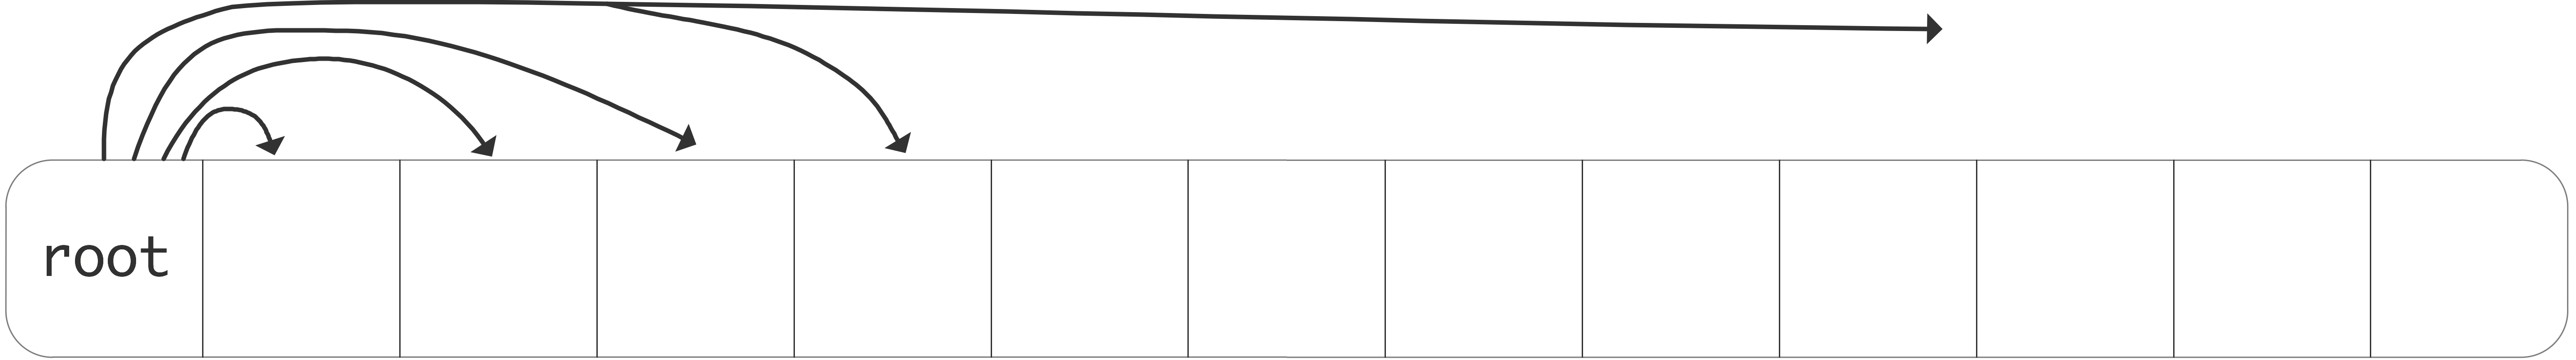
\includegraphics[scale=.08]{graphics-public/bcast-simple}
  \caption{A simple broadcast}
  \label{fig:bcast-simple}
\end{figure}
Typically, it will
be the root of a broadcast tree. You see that there is no message tag,
because collectives are blocking, so you can have only one active at a
time. (In MPI~3 there are non-blocking collectives; see
section~\ref{sec:mpi3collect}.)

It is possible for the data to be an array; in that case MPI acts as if you did a 
separate scalar broadcast on each array index.

If a processor has only one outgoing connection, the broadcast in
figure~\ref{fig:bcast-simple} would take a time proportional to the
number of processors. One way to ameliorate that is to structure the
broadcast in a tree-like fashion.
\begin{figure}[ht]
  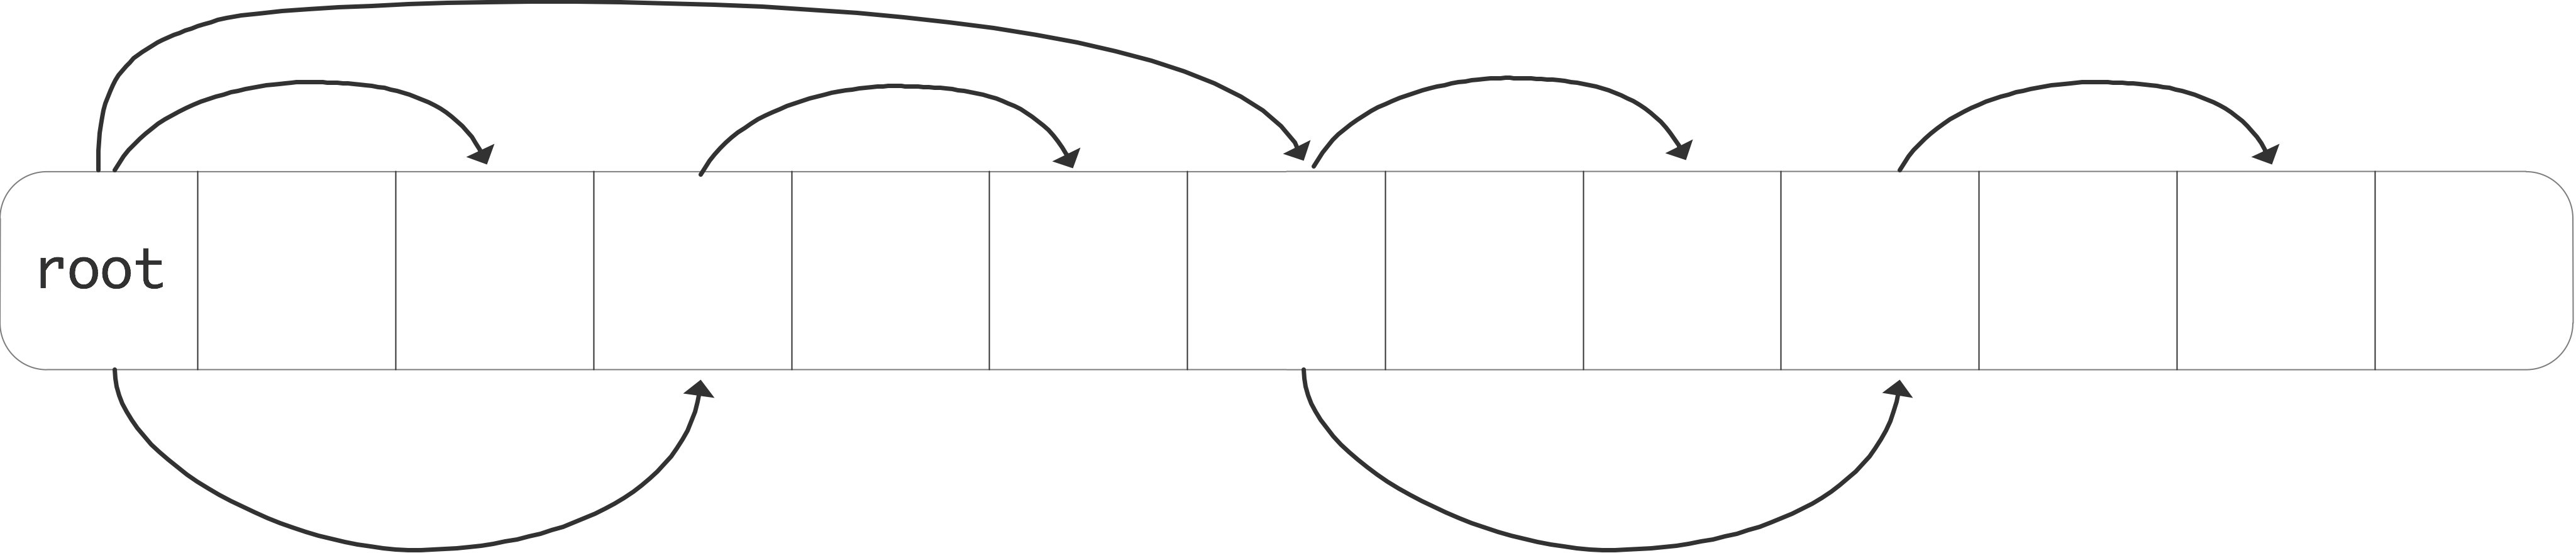
\includegraphics[scale=.1]{graphics-public/bcast-tree}
  \caption{A tree-based broadcast}
  \label{fig:bcast-tree}
\end{figure}
This is depicted in figure~\ref{fig:bcast-tree}. How does the
communication time now depend on the number of processors? The theory
of the complexity of collectives is described in more detail in
\HPSCref{sec:collective}; see also~\cite{Chan2007Collective}.

The reverse of a broadcast is a reduction:
\begin{verbatim}
MPI_Reduce( senddata, recvdata..., operator,
    root, comm ); 
\end{verbatim}
Now there is a separate buffer for outgoing data, on all processors,
and incoming data, only relevant on the root. Also, you have to
indicate how the data is to be combined. Popular choices are
\indexmpishow{MPI_SUM}, \indexmpishow{MPI_PROD} and
\indexmpishow{MPI_MAX}, but complicated operators such as finding the
location of the maximum value exist. You can also define your own operators.

On processes that are not the root, the receive buffer is ignored. On the root, 
you have two buffers, but by specifying \indexmpishow{MPI_IN_PLACE}, the reduction call
uses the value in the receive buffer as the root's contribution to the operation.
On the \n{Allreduce} call, \n{MPI_IN_PLACE} can be used for the send buffer of
every process.

\begin{verbatim}
void *buffer = malloc(size*sizeof(double));
// write data into the buffer
if (mytid==0) {
  sendbuf = MPI_IN_PLACE; recvbuf = buffer;
} else {
  sendbuf = buffer;       recvbuf = NULL;
}
MPI_Reduce(sendbuf,recvbuf,size,MPI_DOUBLE,MPI_MAX,0,comm);
\end{verbatim}

The \indexmpishow{MPI_Scan} operation also performs a reduction, but it keeps 
the partial results. That is, if processor~$i$ contains a number~$x_i$, 
and $\oplus$ is an operator,
then the scan operation leaves $x_0\oplus\cdot\oplus x_i$ on processor~$i$.
\begin{verbatim}
MPI_Scan( send data, recv data, operator, communicator);
\end{verbatim}
This is an inclusive scan operation. The exclusive definition, which computes
$x_0\oplus\cdot\oplus x_{i-1}$ on processor~$i$, can easily be derived
from the inclusive operation for operations such as \n{MPI_PLUS} or \n{MPI_MULT}.
This is not the case for \n{MPI_MIN} or \n{MPI_MAX}, so there is an
exclusive routine
\begin{verbatim}
MPI_Exscan( send data, recv data, operator, communicator);
\end{verbatim}
with the same prototype. 

The \n{MPI_Scan} operation is often useful with indexing data. Suppose that
every processor~$p$ has a local vector where the number of elements~$n_p$ is dynamically 
determined. In order to translate the local numbering $0\ldots n_p-1$ to a global numbering
one does a scan with the number of local elements as input. The output is then the global 
number of the first local variable.

\begin{exercise}
  Do you use \n{MPI_Scan} or \n{MPI_Exscan} for this operation? How
  would you describe the result of the other scan operation, given the
  same input?
\end{exercise}

It is possible to do a \indexterm{segmented scan}. Let $x_i$ be a series of numbers
that we want to sum to $X_i$ as follows. Let $y_i$ be a series of booleans such that
\[ 
\begin{cases}
  X_i=x_i&\hbox{if $y_i=0$}\\
  X_i=X_{i-1}+x_i&\hbox{if $y_i=1$}
\end{cases}
\]
This means that $X_i$ sums the segments between locations where $y_i=0$ and the
first subsequent place where $y_i=1$. To implement this, you need a user-defined operator
\[ 
\begin{pmatrix}  X\\ x\\ y\end{pmatrix}
=
\begin{pmatrix}  X_1\\ x_1\\ y_1\end{pmatrix}
\bigoplus
\begin{pmatrix}  X_2\\ x_2\\ y_2\end{pmatrix}\colon
  \begin{cases}
    X=x_1+x_2&\hbox{if $y_2==1$}\\ X=x_2&\hbox{if $y_2==0$}
  \end{cases}
\]
This operator is not communitative, and it needs to be declared as such
with \indexmpishow{MPI_Op_create}.

\Level 1 {Gather and scatter}

In gather and scatter, the root collects information from, or conversely spreads it to,
all other processes. The difference with reduce and broadcast is that it involves
individual information from/to every process. Thus, the gather operation typically 
has an array of items, one coming from each sending process, and scatter has an array,
\begin{figure}[ht]
  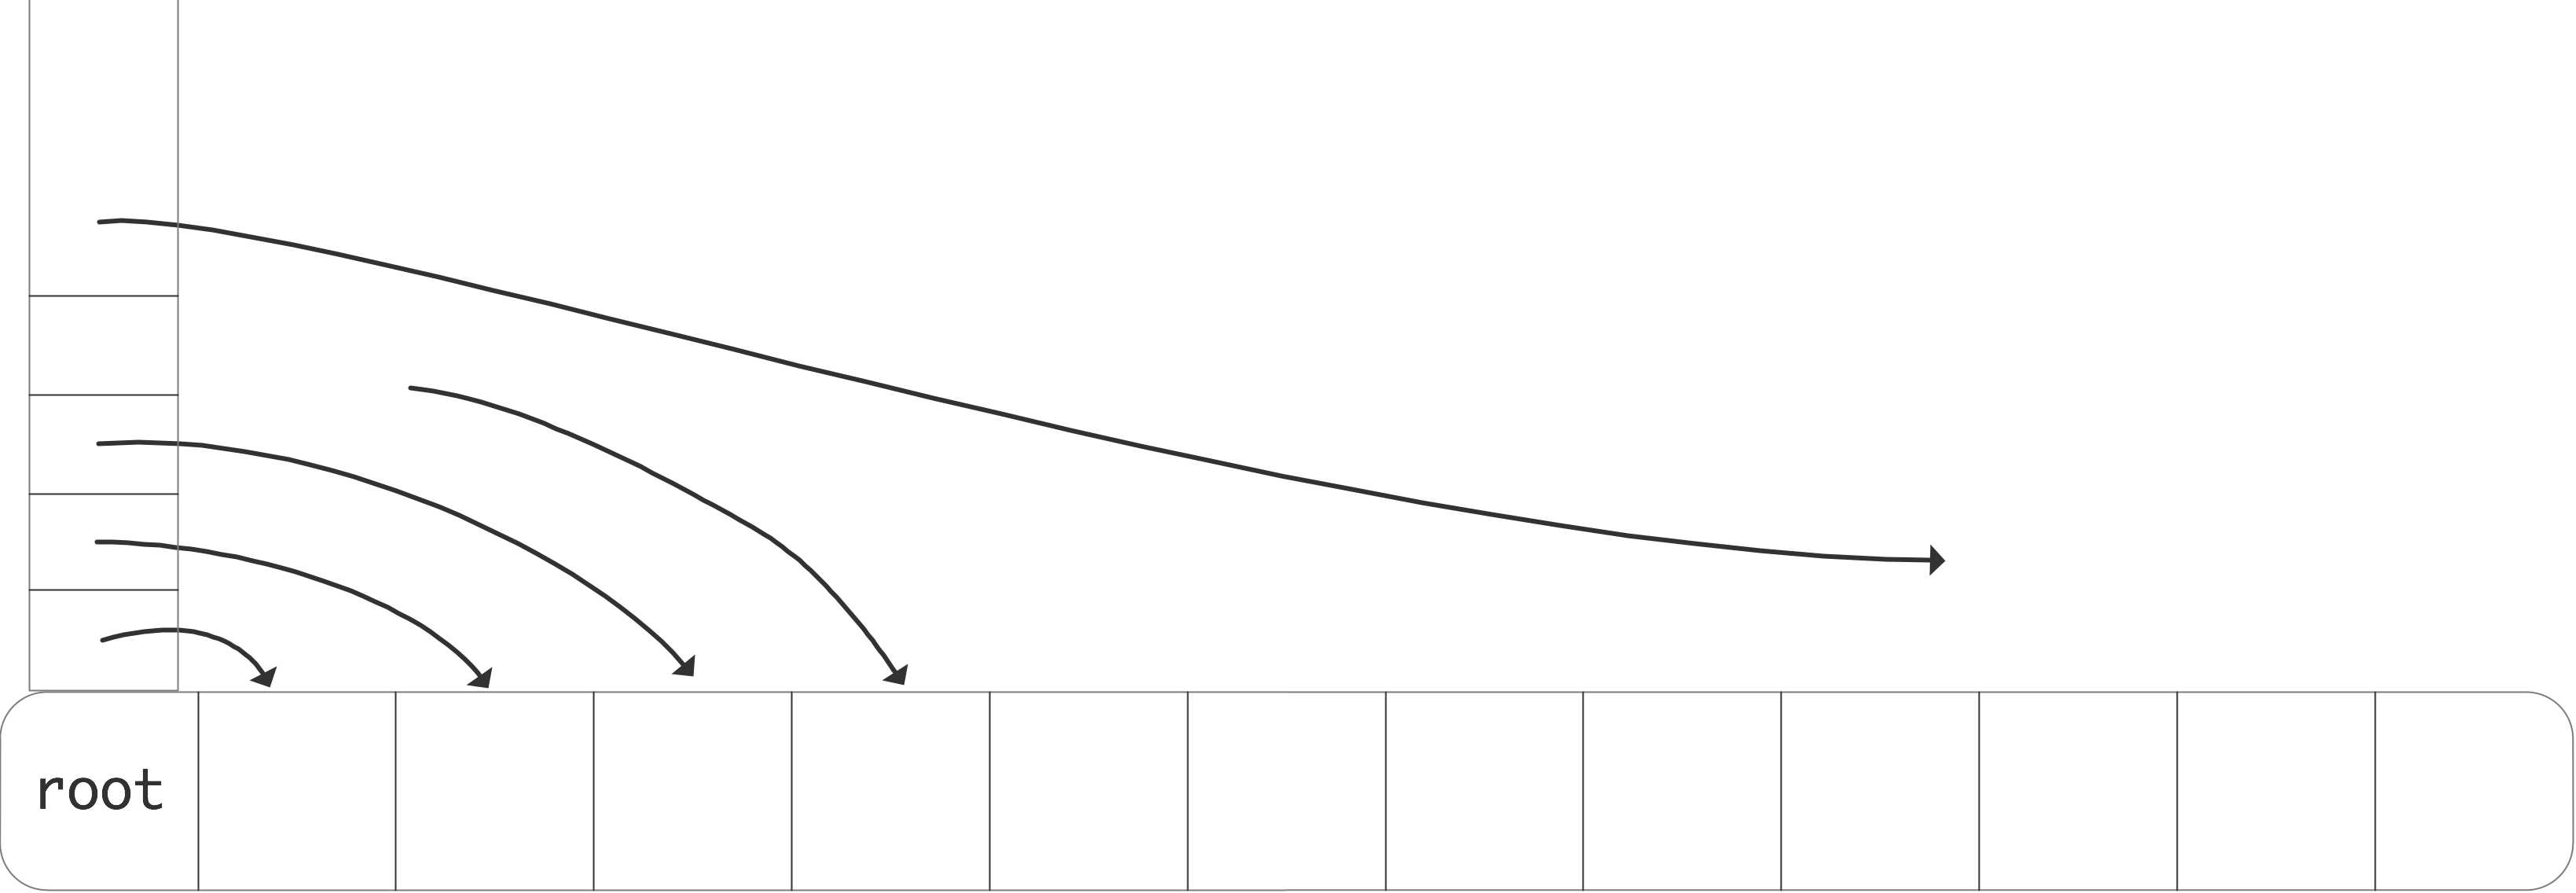
\includegraphics[scale=.12]{graphics-public/scatter-simple}
  \caption{A scatter operation}
  \label{fig:scatter}
\end{figure}
with an individual item for each receiving process; see figure~\ref{fig:scatter}.

To make this more precise, consider, arbitrarily,
the scatter operation. The root process specifies an out buffer:
\begin{verbatim}
outbuffer, outcount, outtype
\end{verbatim}
but the \n{outcount} is not the length of the buffer: it is the number
of elements to send to each process.
On the receiving processes other than the root the outbuffer arguments are irrelevant.

\Level 1 {Variable gather and scatter}

In the gather and scatter call above each processor received or sent
an identical number of items. In many cases this is appropriate, but
sometimes each processor wants or contributes an individual number of
items.

Looking again at the scatter, nothing changes in the receive buffer,
but now the send buffer on the root is more complicated. It now consists of:
\begin{verbatim}
outbuffer, array-of-outcounts, array-of-displacements, outtype
\end{verbatim}

\Level 1 {Non-blocking collectives}
\label{sec:mpi3collect}

MPI version~3 has non-blocking collectives.

\Level 1 {Barrier and all-to-all}

There are two collectives we have not mentioned yet. A~barrier is a
call that blocks all processes until they have all reached the barrier
call. This call's simplicity is contrasted with its usefulness, which
is very limited. It is almost never necessary to synchronize processes
through a barrier: for most purposes it does not matter if processors
are out of sync. Conversely, collectives (except the new non-blocking
ones) introduce a barrier of sorts themselves.

The all-to-all call is a generalization of a scatter and gather: every
process is scattering an array of data, and every process is gathering
an array of data. There is also a `v' variant of this routine.

\Level 1 {Collectives and synchronization}

Collectives, other than a barrier, have a synchronizing effect between processors.
For instance, in
\begin{verbatim}
MPI_Bcast( ....data... root);
MPI_Send(....);
\end{verbatim}
the send operations on all processors will occur after the root executes
the broadcast. 
\begin{figure}[ht]
  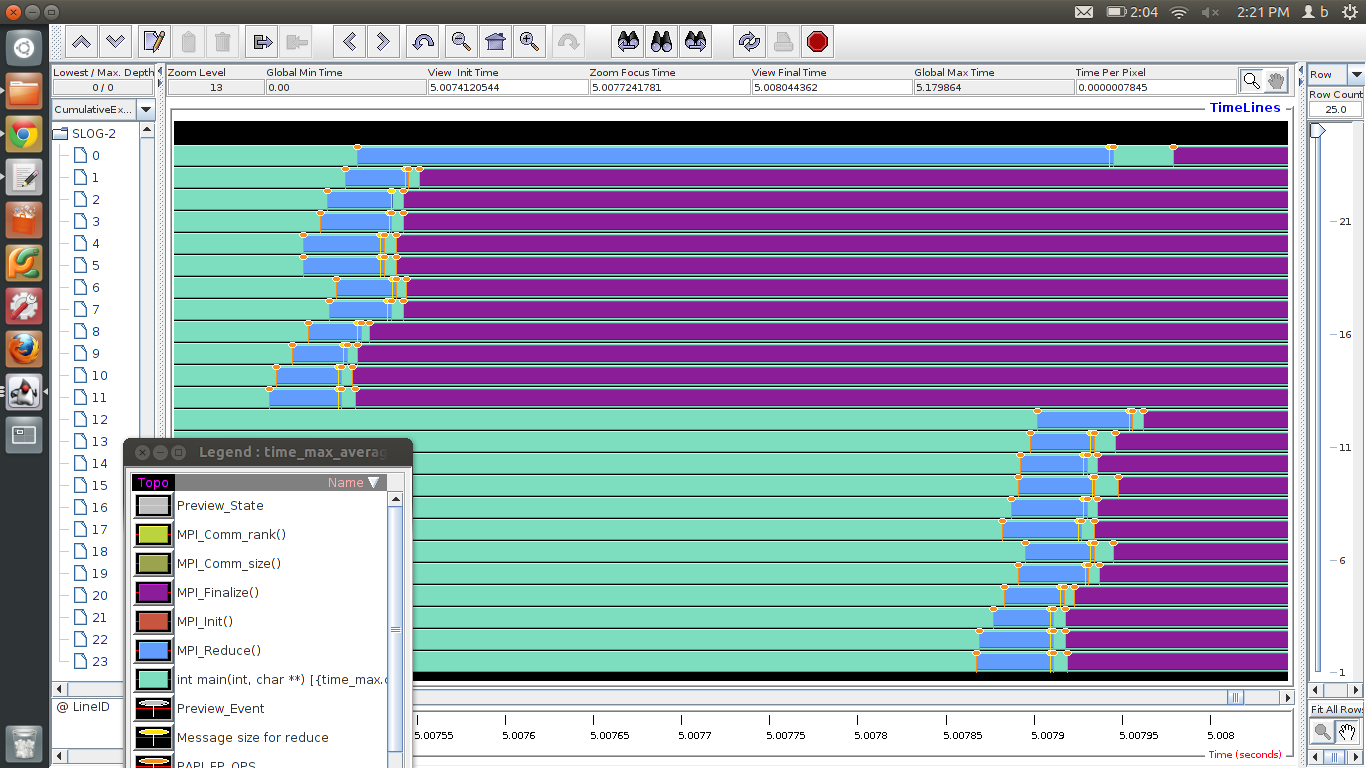
\includegraphics[scale=.35]{graphics-public/reduce-two-node}
  \caption{Trace of a reduction operation between two dual-socket 12-core nodes}
  \label{fig:trace-reduce}
\end{figure}
Conversely, in a reduce operation the root may have to wait for 
other processors. This is illustrated in figure~\ref{fig:trace-reduce}, which 
gives a TAU trace of
a reduction operation on two nodes, with two six-core sockets (processors) each.
We see that\footnote
{This uses mvapich version 1.6; in version 1.9 the implementation of an on-node reduction
has changed to simulate shared memory.}:
\begin{itemize}
\item In each socket, the reduction is a linear accumulation;
\item on each node, cores zero and six then combine their result;
\item after which the final accumulation is done through the network.
\end{itemize}
We also see that the two nodes are not perfectly in sync, which is normal for MPI
applications. As a result, core~0 on the first node will sit idle until it receives the partial
result from core~12, which is on the second node.

While collectives synchronize in a loose sense, it is not possible to
make any statements about events before and after the collectives
between processors:
\begin{verbatim}
...event 1...
MPI_Bcast(....);
...event 2....
\end{verbatim}
Consider a specific scenario:
\begin{verbatim}
switch(rank) { 
    case 0: 
        MPI_Bcast(buf1, count, type, 0, comm); 
        MPI_Send(buf2, count, type, 1, tag, comm); 
        break; 
    case 1: 
        MPI_Recv(buf2, count, type, MPI_ANY_SOURCE, tag, comm, status); 
        MPI_Bcast(buf1, count, type, 0, comm); 
        MPI_Recv(buf2, count, type, MPI_ANY_SOURCE, tag, comm, status); 
        break; 
    case 2: 
        MPI_Send(buf2, count, type, 1, tag, comm); 
        MPI_Bcast(buf1, count, type, 0, comm); 
        break; 
}
\end{verbatim}
Note the \n{MPI_ANY_SOURCE} parameter in the receive calls on processor~1.
One obvious execution of this would be:
\begin{enumerate}
\item The send from~2 is caught by processor~1;
\item Everyone executes the broadcast;
\item The send from~0 is caught by processor~1.
\end{enumerate}
However, it is equally possible to have this execution:
\begin{enumerate}
\item Processor~0 starts its broadcast, then executes the send;
\item Processor~1's receive catches the data from~0, then it executes
  its part of the broadcast;
\item Processor~1 catches the data sent by~2, and finally processor~2
  does its part of the broadcast.
\end{enumerate}

\index{collectives|)}

\Level 0 {Data types}

In many cases the data you send is a single element or an array of some 
elementary type such as byte, int, or real. You pass the data by specifying
the start address and the number of data elements.

Since MPI is a library, and not a language, there is a possibility of 
confusion here: you first declare your variable or array as, say, \n{double},
and subsequently declare it to be \n{MPI_DOUBLE}. First of all, you
can make errors, and the compiler will most likely not catch these.
Secondly, the definition of datatypes is complicated; for instance there
are 32-bit and 64-bit integers. How can you keep your code both 
correct and portable then?

\Level 1 {Elementary data types}

C/C++:
\begin{tabular}{ll}
\n{MPI_CHAR}&only for text data, do not use for small integers\\
\n{MPI_UNSIGNED_CHAR}\\
\n{MPI_SIGNED_CHAR}\\
\n{MPI_SHORT}\\
\n{MPI_UNSIGNED_SHORT}\\
\n{MPI_INT}\\
\n{MPI_UNSIGNED}\\
\n{MPI_LONG}\\
\n{MPI_UNSIGNED_LONG}\\
\n{MPI_FLOAT}\\
\n{MPI_DOUBLE}\\
\n{MPI_LONG_DOUBLE}
\end{tabular}
There is some, but not complete, support for \indexterm{C99} types.

Fortran:
\begin{tabular}{ll}
\n{MPI_CHARACTER}&Character(Len=1)\\
\n{MPI_LOGICAL}\\
\n{MPI_INTEGER}\\
\n{MPI_REAL}\\
\n{MPI_DOUBLE_PRECISION}\\
\n{MPI_COMPLEX}\\
\n{MPI_DOUBLE_COMPLEX}&Complex(Kind=Kind(0.d0))\\
\end{tabular}

\Level 0 {Communicators}

A communicator is an object describing a group of processes. In many 
applications all processes work together closely coupled, and the
only communicator you need is \n{MPI_COMM_WORLD}. However, there are 
circumstances where you want one subset of processes to operate 
independently of another subset. For example:
\begin{itemize}
\item If processors are organized in a $2\times2$ grid, you may want
  to do broadcasts inside a row or column. 
\item For an application that includes a producer and a consumer part,
  it makes sense to split the processors accordingly.
\end{itemize}
In this section we will see mechanisms for defining new communicators
and sending messages between communicators.

An important reason for using communicators is the development of
software libraries. If the routines in a library use their own communicator
(even if it is a duplicate of the `outside' communicator), there
will never be a confusion between message tags inside and outside the 
library.

\Level 1 {Basics}

There are three predefined communicators:
\begin{itemize}
\item \indexmpishow{MPI_COMM_WORLD} comprises all processes that were started 
  together by \indexterm{mpirun} (or some related program).
\item \indexmpishow{MPI_COMM_SELF} is the communicator that contains only
   the current process.
\item \indexmpishow{MPI_COMM_NULL} is the invalid communicator. Routines
  that construct communicators can give this as result if an error occurs.
\end{itemize}
%Implementationally, communicators are integers, so you can use a 
%simple test for equality.

In some applications you will find yourself regularly creating new
communicators, using the mechanisms described below. In that case, you
should de-allocate communicators with \indexmpishow{MPI_Comm_free} when
you're done with them.

\Level 1 {Creating new communicators}

There are various ways of making new communicators. We discuss three 
mechanisms, from simple to complicated.

\Level 2 {Duplicating communicators}

With \indexmpishow{MPI_Comm_dup} you can make an exact duplicate of a communicator.
This may seem pointless, but it is actually very useful for the design of
software libraries. Image that you have a code
\begin{verbatim}
MPI_Isend(...); MPI_Irecv(...);
// library call
MPI_Waitall(...);
\end{verbatim}
and suppose that the library has receive calls. Now it is possible that the 
receive in the library inadvertently
catches the message that was sent in the outer environment.

To prevent this confusion, the library should duplicate the outer communicator,
and send all messages with respect to its duplicate. Now messages from the user
code can never reach the library software, since they are on different communicators.

\Level 2 {Splitting a communicator}

Splittingf a communicator into multiple disjoint communicators
can be done with \indexmpishow{MPI_Comm_split}.
This uses a `colour':
\begin{verbatim}
MPI_Comm_split( old_comm, colour, new_comm, .... );
\end{verbatim}
  and all processes in the old communicator with the same colour
  wind up in a new communicator together. The old communicator still exists,
  so processes now have two different contexts in which to communicate.

Here is one example of communicator splitting. Suppose your processors
are in a two-dimensional grid:
\begin{verbatim}
MPI_Comm_rank( &mytid );
proc_i = mytid % proc_column_length;
proc_j = mytid / proc_column_length;
\end{verbatim}
You can now create a communicator per column:
\begin{verbatim}
MPI_Comm column_comm;
MPI_Comm_split( MPI_COMM_WORLD, proj_j, &column_comm );
\end{verbatim}
and do a broadcast in that column:
\begin{verbatim}
MPI_Bcast( data, /* tag: */ 0, column_comm );
\end{verbatim}
Because of the SPMD nature of the program, you are now doing in parallel
a broadcast in every processor column. Such operations often appear
in \indexterm{dense linear algebra}.

\Level 2 {Process groups}

The most general mechanism is based on groups: you can extract the
group from a communicator, combine different groups, and form a new
communicator from the resulting group.

The group mechanism is more involved. You get the group from a
communicator, or conversely make a communicator from a group with
\indexmpishow{MPI_Comm_group} and \indexmpishow{MPI_Comm_create}:
\begin{verbatim}
MPI_Comm_group( comm, &group);
MPI_Comm_create( old_comm, group, &new_comm );
\end{verbatim}
and groups are manipulated with
\indexmpishow{MPI_Group_incl}, \indexmpishow{MPI_Group_excl},
\indexmpishow{MPI_Group_difference} and a few more.

You can name your communicators with \indexmpishow{MPI_Comm_set_name}, which
could improve the quality of error messages when they arise.

\Level 1 {Intra-communicators}
\label{sec:comm-group}

We start by exploring the mechanisms for creating a communicator that
encompasses a subset of \n{MPI_COMM_WORLD}. 

There is a simple function that splits a communicator into disjoint
communicators:
\begin{verbatim}
MPI_COMM_SPLIT(MPI_Comm comm, int color, int key, MPI_Comm newcomm, ierr)
\end{verbatim}
Each processor specifies what `colour' it is, and processes with the
same colour are grouped into a joint communicator. The `key' value is
used to determine the rank in the new communicator.

The most general mechanism for creating communicators is through
process groups: you can query the group of processes of a
communicator, manipulate groups, and make a new communicator out of a
group you have formed.

\begin{verbatim}
MPI_COMM_GROUP (comm, group, ierr)
MPI_COMM_CREATE (MPI_Comm comm,MPI_Group group, MPI_Comm newcomm, ierr)
\end{verbatim}

\begin{verbatim}
MPI_GROUP_UNION(group1, group2, newgroup, ierr)
MPI_GROUP_INTERSECTION(group1, group2, newgroup, ierr)
MPI_GROUP_DIFFERENCE(group1, group2, newgroup, ierr)
\end{verbatim}

\begin{verbatim}
MPI_GROUP_INCL(group, n, ranks, newgroup, ierr)
MPI_GROUP_EXCL(group, n, ranks, newgroup, ierr)
\end{verbatim}
\begin{verbatim}
MPI_GROUP_SIZE(group, size, ierr)
MPI_GROUP_RANK(group, rank, ierr)
\end{verbatim}

\Level 1 {Inter-communicators}

If two disjoint communicators exist, it may be necessary to
communicate between them. This can of course be done by creating a new
communicator that overlaps them, but this would be complicated: since
the `inter' communication happens in the overlap communicator, you
have to translate its ordering into those of the two worker
communicators. It would be easier to express messages directly in
terms of those communicators, and this can be done with
`inter-communicators'.

\begin{verbatim}
MPI_INTERCOMM_CREATE (local_comm, local_leader, bridge_comm, remote_leader, tag, newintercomm, ierr)
\end{verbatim}
After this, the intercommunicator can be used in collectives such as
\begin{verbatim}
MPI_BCAST (buff, count, dtype, root, comm, ierr)
\end{verbatim}
\begin{itemize}
\item In group~A, the root process passes \n{MPI_ROOT} as
  `root' value; all others use \n{MPI_NULL_PROC}.
\item In group~B, all processes use a `root' value that is the
  rank of the root process in the root group.
\end{itemize}
Gather and scatter behave similarly; the allgather is different: all
send buffers of group~A are concatenated in rank order, and places on
all processes of group~B.

Inter-communicators can be used if two groups of process work
asynchronously with respect to each other; another application is
fault tolerance (section~\ref{mpi:tolerant}).

\Level 0 {Hybrid programming: MPI and threads}\
\commandref{sec:mpi-thread}

It is not automatic that a program or a library is
\indexterm{thread-safe}.  A user can request a certain level of
multi-threading with \indexmpishow{MPI_Init_thread}, and the system
will respond what the highest supported level is.

MPI can be thread-safe on the following levels:
\begin{itemize}
\item An MPI implementation can forbid any multi-threading;
\item it can allow one thread to make MPI calls;
\item it can allow one thread \emph{at a time} to make MPI calls;
\item it can allow arbitrary multi-threaded behaviour in MPI calls.
\end{itemize}

Some points.
\begin{itemize}
\item MPI can not distinguish between threads: the communicator rank
  identifies a process, and is therefore identical for all threads.
\item A message sent to a process can be received by any thread that
  has issued a receive call with the right source/tag specification.
\item Multi-threaded calls to an MPI routine have the semantics of an
  unspecified sequence of calls.
\item A blocking MPI call only blocks the thread that makes it.
\end{itemize}

\Level 0 {Leftover topics}

\Level 1 {Getting message information}

In some circumstances the recipient may not know all details of a message.
\begin{itemize}
\item If you are expecting multiple incoming messages, it may be most
  efficient to deal with them in the order in which they arrive. For
  that, you have to be able to ask `who did this message come from,
  and what is in it'.
\item Maybe you know the sender of a message, but the amount of data
  is unknown. In that case you can overallocate your receive buffer,
  and after the message is received ask how big it was, or you can
  `probe' an incoming message and allocate enough data when you find
  out how much data is being sent.
\end{itemize}

\Level 2 {Status object}

The receive calls you saw above has a status argument. If you 
precisely know what is going to be sent, this argument tells you 
nothing new. However, if you expect data from multiple senders,
or the amount of data is indeterminate, the status will give
you that information.

The \indexmpishow{MPI_Status} object is a structure with the following 
freely accessible members:
\n{MPI_SOURCE}, \n{MPI_TAG}, and \n{MPI_ERROR}. There is also opaque 
information: the amount of data received can be retrieved by 
a function call to \indexmpishow{MPI_Get_count}.
\begin{verbatim}
int MPI_Get_count(
  MPI_Status *status,
  MPI_Datatype datatype,
  int *count
);
\end{verbatim}
This may be necessary since the \n{count} argument to \n{MPI_Recv} is 
the buffer size, not an indication of the actually expected number of
data items.

\Level 2 {Probing messages}

MPI receive calls specify a receive buffer, and its size has to be
enough for any data sent. In case you really have no idea how much data
is being sent, and you don't want to overallocate the receive buffer,
you can use a `probe' call.

The calls \indexmpishow{MPI_Probe}, \indexmpishow{MPI_Iprobe}, accept a message,
but do not copy the data. Instead, when probing tells you that there is a
message, you can use \indexmpishow{MPI_Get_count} to determine its size,
allocate a large enough receive buffer, and do a regular receive to
have the data copied.

\Level 1 {Error handling}
\commandref{mpi:error}

Errors in normal programs can be tricky to deal with; errors in
parallel programs can be even harder. This is because in addition to
everything that can go wrong with a single executable (floating point
errors, memory violation) you now get errors that come from faulty
interaction between multiple executables.

A few examples of what can go wrong:
\begin{itemize}
\item MPI errors: an MPI routine can abort for various reasons, such
  as receiving much more data than its buffer can accomodate. Such
  errors, as well as the more common type mentioned above, typically
  cause your whole execution to abort. That is, if one incarnation of
  your executable aborts, the MPI runtime will kill all others.
\item Deadlocks and other hanging executions: there are various
  scenarios where your processes individually do not abort, but are all
  waiting for each other. This can happen if two processes are both
  waiting for a message from each other, and this can be helped by
  using non-blocking calls. In another scenario, through an error in
  program logic, one process will be waiting for more messages
  (including non-blocking ones) than are sent to it.
\end{itemize}

The MPI library has a general mechanism for dealing with errors that
it detects. The default behaviour, where the full run is aborted, is
equivalent to your code having the following
call\indexmpi{MPI_Comm_set_errhandler}\footnote{The routine
  \n{MPI\_Errhandler\_set} is deprecated.}:
\indexmpi{MPI_ERRORS_ARE_FATAL}\indexmpi{MPI_ERRORS_RETURN}
\begin{verbatim}
MPI_Comm_set_errhandler(MPI_COMM_WORLD,MPI_ERRORS_ARE_FATAL);
\end{verbatim}
Another simple possibility is to specify
\begin{verbatim}
MPI_Comm_set_errhandler(MPI_COMM_WORLD,MPI_ERRORS_RETURN);
\end{verbatim}
which gives you the opportunity to write code that handles the error
return value.

In most cases where an MPI error occurs a complete abort is the
sensible thing, since there are few ways to recover. The second
possibility can for instance be used to print out debugging
information:
\begin{verbatim}
ierr = MPI_Something();
if (ierr!=0) {
    // print out information about what your programming is doing
    MPI_Abort();
}
\end{verbatim}
For instance,
\begin{verbatim}
Fatal error in MPI_Waitall: 
See the MPI_ERROR field in MPI_Status for the error code
\end{verbatim}
You could code this as\indexmpi{MPI_Error_string}\indexmpi{MPI_ERROR}
\begin{verbatim}
MPI_Comm_set_errhandler(MPI_COMM_WORLD,MPI_ERRORS_RETURN);
ierr = MPI_Waitall(2*ntids-2,requests,status);
if (ierr!=0) {
   char errtxt[200];
   for (int i=0; i<2*ntids-2; i++) {
       int err = status[i].MPI_ERROR; int len=200;
       MPI_Error_string(err,errtxt,&len);
       printf("Waitall error: %d %s\n",err,errtxt);
   }
   MPI_Abort(MPI_COMM_WORLD,0);
}
\end{verbatim}
One cases where errors can be handled is that of \emph{MPI file
  I/O}\indexterm{MPI!I/O}: if an output file has the wrong
permissions, code can possibly progress without writing data, or
writing to a temporary file.

\Level 1 {Fault tolerance}
\label{mpi:tolerant}

Processors are not completely reliable, so it may happen that one
`breaks': for software or hardware reasons it becomes
unresponsive. For an MPI program this means that it becomes impossible
to send data to it, and any collective operation involving it will
hang. Can we deal with this case? Yes, but it involves some
programming.

First of all, one of the possible MPI error return codes
(section~\ref{mpi:error}) is \n{MPI_ERR_COMM}, which can be returned
if a processor in the communicator is unavailable. You may want to
catch this error, and add a `replacement processor' to the
program. For this, the \n{MPI_Comm_spawn} can be used:
\begin{verbatim}
int MPI_Comm_spawn(char *command, char *argv[], int maxprocs, MPI_Info info, 
                  int root, MPI_Comm comm, MPI_Comm *intercomm,
                  int array_of_errcodes[])
\end{verbatim}
But this requires a change of program design: the communicator
containing the new process(es) is not part of the
old \n{MPI_COMM_WORLD}, so it is better to set up your code as a
collection of inter-communicators to begin with.

\Level 1 {Profiling}
\label{sec:profile}

\indexmpishow{MPI_Wtime} gives \indexterm{wall clock time} from
unspecified starting point.

\Level 1 {Debugging}
\label{sec:debug}

There are various ways of debugging an MPI program. Typically there
are two cases. In the simple case your program can have a serious
error in logic which shows up even with small problems and a small
number of processors. In the more difficult case your program can only
be run on large scale, or the problem only shows up when you run at
large scale. For the second case you, unfortunately, need a dedicated
debugging tool, and of course the good ones are expensive. In the
first case there are some simpler solutions.

\Level 2 {Small scale debugging}

If your program hangs or crashes even with small numbers of
processors, you can try debugging on your local desktop or laptop
computer:
\begin{verbatim}
mpirun -np <n> xterm -e gdb yourprogram
\end{verbatim}
This starts up a number of X~terminals, each of which runs your
program. The magic of \n{mpirun} makes sure that they all collaborate
on a parallel execution of that program. If your program needs
commandline arguments, you have to type those in every xterm:
\begin{verbatim}
run <argument list>
\end{verbatim}
See appendix~\ref{tut:debug} for more about debugging with~\n{gdb}.

This approach is not guaranteed to work, since it depends on
your \n{ssh} setup; see the discussion
in \url{http://www.open-mpi.org/faq/?category=debugging#serial-debuggers}.

\Level 2 {Large scale debugging}

Check out \indexterm{ddt} or \indexterm{TotalView}.

\Level 2 {Memory debugging of MPI programs}

The commercial parallel debugging tools typically have a memory
debugger. For an open source solution you can
use \indexterm{valgrind}, but that requires some setup during
installation. See \url{http://valgrind.org/docs/manual/mc-manual.html#mc-manual.mpiwrap}
for details.

\Level 1 {Language issues}

MPI is typically written in C, what if you program Fortran?

Assumed shape arrays can be a problem: they need to be copied. 
That's a problem with Isend.

The \indexterm{C++} interface is deprecated as of \indextermbus{MPI}{2.2}.
It is unclear what is happening.

\Level 1 {The origin of one-sided communication in ShMem}

The \indextermbus{Cray}{T3E} had a library called \indexterm{shmem}
which offered a type of shared memory. Rather than having a true
global address space it worked by supporting variables that were
guaranteed to be identical between processors, and indeed, were
guaranteed to occupy the same location in memory. Variables could be
declared to be shared a `symmetric' pragma or directive; their values
could be retrieved or set by \n{shmem_get} and \n{shmem_put} calls.

\Level 0 {Programming projects}
\SetBaseLevel 2
\input projects-public/mpiprojects
\SetBaseLevel 1

\Level 0 {Reference to the routines}

\input chapters-public/mpiref

\Level 0 {Literature}

Online resources:
\begin{itemize}
\item MPI 1 Complete reference:\\ \url{http://www.netlib.org/utk/papers/mpi-book/mpi-book.html}
\item Official MPI documents:\\ \url{http://www.mpi-forum.org/docs/}
\item List of all MPI routines:\\ \url{http://www.mcs.anl.gov/research/projects-public/mpi/www/www3/}
\end{itemize}

Tutorial books on MPI:
\begin{itemize}
\item Using MPI~\cite{Gropp:UsingMPI1} by some of the original authors.
\end{itemize}

\endinput

Examples: 
compute pi
mandelbrot set
